\documentclass[12pt,onesided]{amsart} 

%%%%%%%%%%%%%%%%%%%%%%%%%%%%%%%%%%%%%%%%%%%%%%%%%%
%%%%%%%%%%%%%%%%%%%% PREAMBLE %%%%%%%%%%%%%%%%%%%%
%%%%%%%%%%%%%%%%%%%%%%%%%%%%%%%%%%%%%%%%%%%%%%%%%%


% -------------------- defaults -------------------- %
% load lots o' packages

% layout control
\usepackage{geometry}
\geometry{verbose,tmargin=1.25in,bmargin=1.25in,lmargin=1.1in,rmargin=1.1in}
\usepackage{rotating}
\usepackage{fancyhdr}
\usepackage{parallel}
\usepackage{parcolumns}
%\usepackage{abstract}
%\renewcommand{\abstractname}{}    % clear the title
%\renewcommand{\absnamepos}{empty} % originally center

% math typesetting
\usepackage{array}
\usepackage{amsmath}
\usepackage{amssymb}
\usepackage{amsfonts}

% tables
\usepackage{tabularx}
\usepackage{booktabs}
\usepackage{multicol}
\usepackage{multirow}
\usepackage{longtable}

\usepackage[%
decimalsymbol=.,
digitsep=fullstop
]{siunitx}

% to adapt caption style
\usepackage[font={small},labelfont=bf]{caption}

 
% references
\usepackage[longnamesfirst]{natbib}
\bibpunct{(}{)}{;}{a}{}{,}
\usepackage{nameref}

% footnotes at bottom
\usepackage[bottom]{footmisc}

% to change enumeration symbols begin{enumerate}[(a)]
\usepackage{enumerate}

% to make enumerations and itemizations within paragraphs or
% lines. f.i. begin{inparaenum} for (a) is (b) and (c)
\usepackage{paralist}

% to colorize links in document. See color specification below
\usepackage[x11names]{xcolor}

% for multiple references and insertion of the word "figure" or "table"
% \usepackage{cleveref}

% load the hyper-references package and set document info
\usepackage[pdftex]{hyperref}

% graphics stuff
\usepackage{subfig}
\usepackage{graphicx}
\usepackage[space]{grffile} % allows us to specify directories that have spaces
\usepackage[section]{placeins} % prevents floats from moving past a \FloatBarrier or section
\usepackage{tikz}
% \usepackage{pgfplots}

\usepackage{endfloat}

% Spacing
\usepackage[doublespacing]{setspace}

% define clickable links and their colors
\hypersetup{
	unicode=false,          % non-Latin characters in Acrobat's bookmarks
	pdftoolbar=true,        % show Acrobat's toolbar?
	pdfmenubar=true,        % show Acrobat's menu?
	pdffitwindow=false,     % window fit to page when opened
	pdfstartview={FitH},    % fits the width of the page to the window
	pdfnewwindow=true,%
	% pdfauthor={Cassy Dorff and Shahryar Minhas},%
	pdftitle={Title},%
	colorlinks,%
	citecolor=black,%
	filecolor=black,%
	linkcolor=black,%
	urlcolor=RoyalBlue4%
	}

% Including External Code
\usepackage{verbatim}
\usepackage{listings}
\lstset{
	language=R,
	basicstyle=\scriptsize\ttfamily,
	commentstyle=\ttfamily\color{gray},
	numbers=left,
	numberstyle=\ttfamily\color{gray}\footnotesize,
	stepnumber=1,
	numbersep=5pt,
	backgroundcolor=\color{white},
	showspaces=false,
	showstringspaces=false,
	showtabs=false,
	frame=single,
	tabsize=2,
	captionpos=b,
	breaklines=true,
	breakatwhitespace=false,
	title=\lstname,
	escapeinside={},
	keywordstyle={},
	morekeywords={}
	}
	
\usepackage{etoolbox}

\makeatletter
\patchcmd{\@settitle}{\uppercasenonmath\@title}{}{}{}
\patchcmd{\@setauthors}{\MakeUppercase}{}{}{}
\patchcmd{\section}{\scshape}{}{}{}
\makeatother

\usepackage{caption}
\captionsetup[FLOAT_TYPE]{labelsep=empty}

% -------------------------------------------------- %


% -------------------- title -------------------- %

\title{When Do States Say Uncle? Network Dependence and Sanction Compliance\\}

\author{Cassy Dorff\\
\textit{University of New Mexico}\\
and\\
Shahryar Minhas\\
\textit{Duke University}}

% \date{Draft Copy \today}

% \author[Dorff]{Cassy Dorff}
% \address{Cassy Dorff: Department of Political Science}
% \curraddr{Duke University, Durham, NC, 27708, USA}
% \email{cassy.dorff@duke.edu}
%
% \author[Minhas]{Shahryar Minhas}
% \address{Shahryar Minhas: Department of Political Science}
% \curraddr{Duke University, Durham, NC, 27708, USA}
% \email{shahryar.minhas@duke.edu}

 \thanks{$^{1}$This paper was prepared for 72$^{nd}$ annual Midwest Political Science Association Conference in Chicago, April 2-6 2014. We are grateful for comments on earlier versions of this paper received at the ISSS-ISAC Conference in Washington, D.C., October 4-6 2013. This publication was made possible (in part) by a grant from the Carnegie Corporation of New York. The statements made and views expressed are solely the responsibility of the author. Alphabetical order implies equal authorship, all mistakes are our own.}

\setlength{\headheight}{15pt}
\setlength{\headsep}{20pt}
\pagestyle{fancyplain}
 
\fancyhf{}
 
\lhead{\fancyplain{}{\textit{Network Dependence and Sanction Compliance}}}
\chead{\fancyplain{}{}}
\rhead{\fancyplain{}{Cassy Dorff and Shahryar Minhas}}
\rfoot{\fancyplain{}{}}

% ----------------------------------------------- %


% -------------------- customizations -------------------- %

% define the includegraphics search path
% \graphicspath{{Graphics/}}

% easy commands for number propers
\newcommand{\first}{$1^{\text{st}}$}
\newcommand{\second}{$2^{\text{nd}}$}
\newcommand{\third}{$3^{\text{rd}}$}
\newcommand{\nth}[1]{${#1}^{\text{th}}$}

% easy command for boldface math symbols
\newcommand{\mbs}[1]{\boldsymbol{#1}}

\graphicspath{{/Users/s7m/Dropbox/Research/Magnesium/Graphics/}, {/Users/janus829/Dropbox/Research/Magnesium/Graphics/}, {/Users/cassydorff/Dropbox/Research/Magnesium/Graphics/}}

% -------------------------------------------------------- %


%%%%%%%%%%%%%%%%%%%%%%%%%%%%%%%%%%%%%%%%%%%%%%%%%%
%%%%%%%%%%%%%%%%%%%% DOCUMENT %%%%%%%%%%%%%%%%%%%%
%%%%%%%%%%%%%%%%%%%%%%%%%%%%%%%%%%%%%%%%%%%%%%%%%%

\doublespacing 

\begin{document}
\renewcommand{\abstractname}{ }
\maketitle\thispagestyle{empty}

\begin{abstract}
\abstractname{}
\singlespacing{In this article we address the long-debated question of when and why states comply with sanctions. While the literature remains indeterminate as to whether the key mechanisms driving sanction compliance are tied to interstate relations, intrastate constraints, or a dynamic combination of the two, our theoretical framework and methodological approach provides a novel perspective that incorporates insights drawn from network theory to explain the time until countries comply. Specifically, we argue that reciprocity, a concept with deep roots in both network theory and international relations, has largely been overlooked in the study of sanction compliance. Though ignored this concept captures an essential aspect of how cooperation is fostered in the international system, and allows us to better capture the strategic environment underlying sanctioning behavior. Given the theoretical importance of reciprocity in understanding interstate relations, we provide an approach that integrates estimations of this type of network interdependency into extant frameworks for empirically estimating the time until countries comply with sanctions. Our results highlight that not only does reciprocity have a substantive effect in explaining the duration of sanctions, but that models excluding this concept from their specifications do notably worse in terms of their predictive performance.\\

\noindent \textit{Word Count: 8,668}}

\end{abstract}

\newpage\setcounter{page}{1} 

%%%%%%%% INTRO %%%%%%%%
%\section*{Introduction}
\label{intro}

Economic sanctions are a frequently used foreign policy tool in the realm of international relations. Typically, one or more states initiate sanctions against another to force the target state to change policy. Policy change is expected to occur by depriving the sanction target of trade or other forms of economic exchange with the sanction initiator(s). Triggers for economic sanctions can occur in many contexts: the target state breaks a previous agreement, the target state openly disobeys international law, or the target state engages in behavior that is simply unfavorable to the political preferences of another state. The consequences of sanctions for the populations in target countries can be severe, including increased unemployment, foreign investment loss, and reduced trade flows \citep{hufbauer2003impact,hufbauer1997us}. 

Economic disruption is the general intent of economic sanctions, as Woodrow Wilson told the United States Senate sanctions are a ``peaceful, silent deadly remedy'' for coercing concessions from other states \citep{foley23}. However, motivations for sanction initiation are cross-cutting, spanning a diverse and interdependent mix of policy issues and political actors. Though sanctions often succeed in disrupting economic activity in target states \citep{escriba2010dealing}, their ability to force policy change is debated among both policymakers and scholars.  While the concept of sanctions -- the idea that countries can pressure each other via economic ties in order to influence policy -- is relatively straightforward, the study of when and why sanctions work is complex. While early research argued that sanctions have little influence on targets,\footnote{\cite{lam1990, dashti1997, morgan1997, drezner1998}} more recent work suggests that the effectiveness of sanctions is dependent on the interaction of several factors, namely: the number of senders sanctioning a target state and the type of issue in dispute;\footnote{\cite{miers2002, morgan2009threat}} the strength of domestic institutions within the target state;\footnote{\cite{dashti1997,marinov2005}} and the type of regime governing the target state.\footnote{\cite{mcgillivray2004,lektzian2007,allen2008domestic}} 

We argue that scholars fall short in incorporating a key factor into their analysis of the time until sanctions end in compliance: reciprocity.\footnote{Previous work by \cite{cranmer2014reciprocity} has highlighted the role that network effects such as reciprocity have in the creation of new sanctions, but they also did not address issues of compliance.} Drawing on the work in international relations on trade and conflict, we suggest that sanction cases are best conceptualized as a network phenomenon and should be addressed both theoretically and empirically in these terms. Reciprocity is not a new concept to the field of international studies, but has its roots in previous theories of cooperation and the evolution of norms between states.\footnote{\cite{richardsonai:1960,choucri:north:1972,goldstein1991reciprocity,ward1992reciprocity}} 

% However, the sanction literature has not yet addressed whether reciprocity plays a role in driving states' strategic calculation to comply with a sanction. % repetitive

We posit that the structure created by reciprocal interactions over time should be accounted for in studies of sanction outcomes, and provide a framework through which to estimate these second order dependencies. Further, we incorporate our measures of reciprocal interactions into a duration modeling framework, thus enabling us to explicitly account for interdependencies in the time building up to the resolution of sanctions. In doing so we also test key hypotheses from the literature and assess the extent to which factors such as domestic political institutions and internal stability influence sanction duration once network dynamics are incorporated.  

In the following section, we review previous work on compliance and introduce the network concept. We then present our central argument and hypothesis, while doing so we explain how networks can be conceptualized in this context. Last, we present our findings and review the results.

% International law, in this sense, exists in a state of nature - there is no overarching legal authority with compulsory jurisdiction to enforce agreements. Inevitably, reciprocity has become an important element in the practice of sovereign nations and in the body of existing international law.
%%%%%%%%%%%%%%%%%%%%%%%

%%%%% Lit Review %%%%%
\subsection*{When do Sanctions End?}
\label{lit}

Previous work on the duration of sanctions, or when and why a target state will decide to comply with a particular sanction, has focused on both intrastate and interstate arguments, with an emphasis on the role that domestic factors play in preventing or promoting the efficacy of sanctions. \cite{marinov2005} argues that sanctions ``work'' by directly destabilizing heads of states. Accordingly, destabilization of leaders is a necessary condition for successful coercion.  This focus on internal state conditions echoes other work suggesting that sanction outcomes are dependent on domestic stability and institutions. For example, {\cite{dashti1997}} argue that if a regime is already experiencing a high level of internal conflict, such as protests or violent clashes, the onset of an economic sanction restricting trade would further weaken the regime. This heightens the cost of resistance against the sanction \citep{dashti1997}. 

Similarly, \cite{dorussen2001} suggest that domestic support determines the duration (or ``ending'') of sanctions. They argue that when target states' domestic constituencies support resistance against sanctions, leaders have greater incentives to not comply with the sanction, which effectively increases the sanction's duration. Further supporting the idea that domestic institutions condition whether and when states comply with sanctions, \cite{lektzian2007} finds that differing institutional incentives between nondemocratic regimes than democratic ones influence the success of economic sanctions. \cite{mcgillivray2004} employ a hazard model to analyze a data set of 47 sanctions cases. They find that leadership change does strongly influence the duration of sanctions, but only in the case of non-democratic states. Similarly, \cite{bolks2000} consider the determinants of economic sanction duration, but these authors also restrict themselves to target state characteristics in determining time until compliance. These authors also look inside the target state to define domestic conditions that influence sanction outcome. They suggest that the ``decision-making'' environment can either hinder or help the leader take countermeasures against the sanction. This ``decision-making'' environment is affected by factors such as a lack of coordination between government actors and local instability. 

The literature has clearly argued that domestic conditions are an influential predictor of sanction compliance. Yet, other factors are also important to the decision-making environment: critical is the relationship between sanctioning states and target states. Specifically, research must address how key dependencies between countries inform the strategic environment of states through an evolution of behavior in trade relations, ally ties, or geographic proximity over time; and how this complex, evolving strategic environment affects sanction outcomes \citep{mclean2010friends}. Each relationship between the sanctioner and the sanctioned takes on a slightly different influence dependent on these factors. For example, if a neighboring state is greatly dissatisfied with the target's behavior, than a conflict of interest could have more serious repercussions than for a sanctioner who is geographically removed from the target. These types of external factors characterize group level dynamics that exist within each sanction case. 

Recent work has also successfully paired modeling techniques with theoretical prepositions by utilizing hazard-based duration models. The extant literature has demonstrated that this approach more accurately captures the important time-variant dynamics relevant to understanding the sanction process \citep{bolks2000}. Clearly, if the goal of research is to both explain and predict when a target state is likely to comply to a sanction, then researchers have clear incentives to include time-variant data. Using a duration modeling approach allows for the assessment of whether a specific factor, such as political instability or regime type, increases or decreases the probability that a target country will comply with a sanction over time.

While it is intuitive to many researchers that trade dependence between target and sender states likely influences the duration of economic sanctions, and that domestic conditions influence the target's behavior, these previous studies do not fully incorporate the evolution of interaction between states over time. Interactions between actors over time can be captured by a network approach, which can provide a deeper understanding of how the history of sanctions and compliance between states influences future behavior vis-\`a-vis compliance. Further not accounting for possible interdependencies can cause inappropriate empirical inferences \citep{erikson2014dyadic}. \citet{cranmer2014reciprocity} also argue that the sanction literature has not yet accounted for network dynamics, and provide a network based model to explore sanction initiation. They demonstrate that the \textit{onset} of sanctions are best predicted by modeling the way in which interdependencies evolve over time and influence the future decisions made by states. \citet{hafner2008} also study sanction onset via a networked approach and show that increases in bilateral trade decrease sanctioning behavior between states.

Critical concepts like these are currently ignored in the research on sanction compliance. By avoiding network attributes, researchers miss a wealth of structural information that is critical to understanding the ebb and flow of international cooperation and conflict.\footnote{The insight that the international system is inherently a network and must be studied as such has gained increasing theoretical and empirical support in the broader international relations literature; most prominent is the work on trade networks,\cite{hoff2004modeling, ward:rainbow:2013} conflict,\cite{AnneAuthor} alliances,\cite{warren2010geometry} and intragovernmental organizations.\cite{cao2009networks,greenhill2010norm}} We provide a way to account for these network interdependencies within the context of a simple duration model.

%Furthermore, current duration approaches are unable to account for the history of dependencies between countries over time, and thus ignore previous cases of compliance and sanction interdependence between target and sanctioning states.  Over time, complex interdependencies likely emerge and drive behavior between states, where if country \textit{i} complies often to country \textit{j}, country \textit{j} might also be more likely to comply to country \textit{i}. This process is typically known as reciprocity, and is one of the key network attributes we account for in our analysis below. 



%%%%%%%%%%%%%%%%%%%%%%

%%%%% Theory %%%%%
\section*{Reciprocity \& Network Effects}
\label{neteffects}

A common analogy in the coercive diplomacy literature centers on the contrast between ``sticks'' and ``carrots''. When applied to the economic sanctions literature, this analogy frames economic sanctions as sticks, and economic incentives as carrots. Countries often use sanctions as sticks with those to whom they share various strategic ties to resolve trade related disputes.  Compliance in sanction cases involving actors with strong strategic ties to one another are often assumed to be more assured because it is unlikely that the involved countries would risk jeopardizing their positive relations with one another. However, this comes with an important caveat: we argue that compliance is not just dependent on individual ties based on unidimensional concepts such as trade, but that compliance is dependent the previous strategic interactions between actors. The process of sanction compliance is thus driven by this endogenous evolution between states' shared strategic environment and past reciprocal behavior.

In studies of social and economic behavior, direct reciprocity -- the notion that actors learn to ``respond in kind" to one another -- is argued to be an essential component of behavior.\footnote{For example, see \cite{bolton:1998, charness:2002, charness:2004, cox:2007, cox:2004}.} The idea that individuals, or collectives, observe previously cooperative (or conflictual) behavior from others, and include this information into their own decision-making process, is a concept given great value to determine strategic outcomes. For example, reciprocity is shown to influence interactions across diverse settings including tax compliance \citep{smith:1990}, wage selection \citep{campbell:1997}, and strike breaking \citep{brett:1998}. Reciprocity is also shown to play a critical role in the development of interethnic attitudes whereby groups tend to reflect the attitudes that other groups hold toward them \citep{berry:1979}. 

International Relations (IR) scholars have long argued that given the anarchic nature of the international system reciprocity is critical to the evolution of cooperative and conflictual interactions among states \citep{keohane1989reciprocity}. This assertion dates back to early research on foreign policy. Scholars concerned with understanding the onset of World War I acknowledged the importance of tit-for-tat interactions \citep{holsti1972}. \cite{rajmaira:1990} argue that reciprocity determines long-term foreign policy behavior among superpowers. In other realms of international politics, reciprocity plays a key role in formulating expectations of state behavior. As one scholar notes, ``It is an empirical datum that people tend to respond to others with an implicit policy of like for like and that this facilitates cooperation between them. This elementary fact has profound implications for the effective design of law and institutions.'' \cite[p. 19]{osiel:2009}. Reciprocity has long been recognized by IR scholars as an important mechanism for the enforcement of agreements and instantiation of cooperation. 
	
% This same logic is rooted in research investigating the �iterated prisoner�s dilemma.\cite{axelrod:1985} outline the basic logic of reactive response in repeated interactions and highlights how reciprocal interactions foster cooperation. 

While reciprocity receives little attention in sanctions research, much of the literature instead focuses on how specific types of relationships between senders and targets -- such as alliances and trade ties -- expedite sanction resolution. The core mechanisms driving sanction outcomes are thus characterized in terms of a cost-benefit analysis, ignoring the plausible role that learning plays in driving state behavior. Underlying the exogenous relational dimensions explored in the literature is the concise argument that there are some set of countries from whom the sending of sanctions are more consequential, and will thus be complied to more quickly, than others. However, by ignoring reciprocity the extant analyses of these linkages disregards the history of interactions between two countries. We argue that reciprocal interactions provide a fundamental reflection of the strategic environment that shapes state's compliance behavior. More specifically, we posit that reciprocity influences sanction outcomes through two key processes: behavioral expectations formed and information sharing. 

The first process is that which is promoted by existing work on reciprocity and cooperation: one actor has incentive to ``respond in kind'' to the previous behavior of their partner. In international relations, states that are perceived as cooperative will be more likely to have future partners cooperate with them, and in the same timely or untimely manner. The concept of information sharing has received a great deal of attention in the international bargaining literature, and the sanctioning process has often been conceptualized as a form of international bargaining.\footnote{For example, see \cite{morgan1999threats,lacy2004theory,marinov2005}.} In any sanction case, there is uncertainty about the target state's willingness and capacity to endure the sanction.  Anytime a sanction is endured, information is shared between states as both the sender and target state decide how to respond to one another's behavior. During this time, each state reveals more information about their preferences and resolve. We argue that the evolution of ties between sender and target states influences the calculation states make over time through revealing previously unknown preferences for cooperation. 

Overtime, this learning mechanism--made possible by reciprocity--informs the target state's decision to comply more swiftly, or to delay compliance to show resolve rather than cooperation. Our basic intuition is to expect that when a target state has a richer history of reciprocal compliance with sender states, they will more swiftly comply with the senders' demands. 

% SHOULD WE INCLUDE SOMETHING LIKE THIS? I don't think so: Furthermore, it is key to consider how this concept is important when we conceptualize sanctions as a networked process. Imagine a scenario in which Iran signals to the United States, via sanctions, that the U.S is engaging in unfavorable policy to Iran. In the past, these two countries have little history of a shared, reciprocal history of compliance. However, if a nation like Canada sanctions the U.S., most likely the U.S. will carefully consider its response. Finally, if Canada, and the United Nations, Australia, and Sweden join together to sanction the U.S. for disagreeable actions, the U.S. is likely to very seriously consider compliance in a timely manner. This is not a simple, one-shot cost-benefit analysis, but instead is explained by a previous history of strategic interaction between the target state, and the network of sender states. % SM : I think this would get us into trouble and people would immediately think of other reasons for the theoretical example we provide above, trade ties is one that quickly comes to mind. 

\subsection*{Measuring Reciprocity}

Before we describe our procedure for measuring reciprocity, we provide a glimpse of why sanctions need to be thought of in a network context. Figure \ref{fig:spaghetti} depicts the network of sanction cases on-going and initiated by 1984. This network graph presents the entire sanction-year network.  Nodes represent states and the directed edges denote the sender and receiver of sanctions. This figure is complex, showing that each yearly network contains important information about state behavior, whereby numerous states are involved in multiple sanction cases during this individual year. Extant analyses on sanction duration do not capture sanction-year attributes and ignore how network characteristics evolve over-time to inform future behavior within sanction networks. While studies of international relations tend to recognize the interdependent nature of state behavior in the theoretical sense, they often fail to uphold this theoretical intuition in empirical analysis. Early attempts are noteworthy,\footnote{\cite{keohane1989reciprocity,goldstein1991reciprocity}} and more recent work has continued to address this concern,\footnote{\cite{mitchell2001,cranmer2014reciprocity}} yet studies on sanction compliance have not incorporated these insights. 

\begin{figure}[ht]
  \centering
  \begin{tabular}{c}
	  \includegraphics[width=1\textwidth]{84net-crop} \\
	  \includegraphics[width=0.45\textwidth]{MapLegend}
  \end{tabular}
  \caption{Here we show the sanction network in 1984, nodes are colored by geographic coordinates of countries. Data for sanction cases comes from \citet{morgan2009threat}.}
  \label{fig:spaghetti}
\end{figure}
\FloatBarrier

We develop two reciprocity concepts to analyze the interdependencies inherent in the evolution of sanction dynamics: \textit{compliance reciprocity} and \textit{sanction reciprocity}. We first outline the compliance reciprocity measure. This measure represents a target states' cumulative history of compliance with a particular sender relative to all others in the network. Our measure of compliance reciprocity allows us to capture whether those who have a history of cooperative behavior with each other also tend to have more cooperative behavior in the future. In a duration context, states who receive sanctions from those with whom they have a history of reciprocal compliance are likely to comply sooner, than they would with lower states to whom they have not had positive reciprocal interactions. 

Notably, this measure is distinct from a simple counter of past instances of compliance with another state. Such a measure would completely ignore the fact that each state's actions are conditional on all other interactions between states. For example, if state $i$ complies often to state $j$, is state $i$ also more likely to comply with all other partner states? Or, relative to all other interactions, does state $i$ comply more frequently and uniquely with state $j$? The latter idea is the one explicated within our  concept of compliance reciprocity. Thus, reciprocity tells us information about the behavior between country $i$ and $j$ over time, relative to how country $i$ interacts with all other partners over time. 

To operationalize our measure of reciprocity, we turn to the Social Relations Model developed by \citet{kenny1994interpersonal}. To illustrate, consider the matrix $X_{ij}$ below, in which we have six actors in a round robin (dyadic) format. These data are represented by the matrix below, which has a value for each of the thirty interactions, with the main diagonal remaining empty:

\singlespacing
\[
\left[
\begin{array}{cccccc}
 & X_{12}  & X_{13}  & X_{14} & X_{15} & X_{16} \\
X_{21}  &  & X_{23}  & X_{24} & X_{25} & X_{26} \\
X_{31}  & X_{32}  &    & X_{34} & X_{35} & X_{36} \\
X_{41}  & X_{42}  & X_{43}  &  & X_{45} & X_{46} \\
X_{51}  & X_{52}  & X_{53}  & X_{54} &   & X_{56} \\
X_{61}  & X_{62}  & X_{63}  & X_{64} & X_{65} &   \\
\end{array}
\right]
\]

\doublespacing
First, we begin with calculating the row column and total sums:

\begin{itemize}
	\item The totals for each \emph{ row} are denoted $X_{i \cdot}$ where $i$ is the row number, i.e.,
	~\\
	$X_{i \cdot} = \sum_{j=1}^{J} X_{ij}$;
	\item For each column the totals are denoted
	 $X_{\cdot i}$ where $i$ is the \emph{column} number; and 
	 \item The total over all rows and columns is given by $X_{\cdot \cdot} = \sum_i \sum_j X_{i,j}$.
 \end{itemize}
 
Given these quantities, one can calculate individual effects for a variety of concepts, such as the actor, partner, and unique dyadic effects, (as well as the variances attributed to each of these effects). The unique dyadic effects, or the reciprocal interactions between two countries within one pair, are calculated accounting for the general behavior of each country within the pair. Or, in other words, this measure captures how likely country $i$ is to comply with country $j$; and the likelihood that country $j$ is to comply with country $i$ is calculated relative to how often country $i$ tends to comply with all of the other countries, as well as how likely country $j$ is to comply with all others. 

 \begin{itemize}
	 \item The actor effect for observation $i$ is the total of $i$'s row mean and column mean, minus the overall mean.  The means are just the sums, corrected for degrees of freedom, yielding an average row effect:\\
	 $\hat{a}_i = \frac{(n-1)^2}{n(n-2)} X_{i \cdot} + \frac{(n-1)}{n(n-2)} X_{\cdot i} -  \frac{n-1}{n-2} X_{\cdot \cdot} $
	\item Similarly the column mean for actor $i$ is \\
	 $\hat{b}_i = \frac{(n-1)^2}{n(n-2)} X_{\cdot i} + \frac{(n-1)}{n(n-2)} X_{i \cdot } -  \frac{n-1}{n-2} X_{\cdot \cdot} $.\\ For a symmetric matrix, the row effect and the column effect will be identical.
	\item The unique dyadic effect, or reciprocity for specific dyad $ij$, simply subtracts the row and column effects along with the overall mean out of the value for dyad $ij$. \\
	$\hat{g}_{ij} = X_{ij} - \hat{a}_i - \hat{b}_j - X_{\cdot \cdot}$
 \end{itemize}

\doublespacing
The first two equations show how the final equation for reciprocity is calculated relative to the general actor and partner effects (or actor and partner average behavior) for each country.\footnote{\cite{kenny1994interpersonal} would suggest including the full compliment of the SRM into our model. We originally explored this approach, but gained little empirical leverage from it, and thus focus instead on the concept of reciprocity.} In figure \ref{fig:recipNet}, we provide a visualization of the \textit{compliance reciprocity} measure generated using the approach laid out above for 1972, 1992, and 2012. In each panel, we include the reciprocity scores for the ten countries that were most active in the sanctioning network at that year. Each of the edges are directional and indicate how likely a country is to reciprocate compliance from another; reciprocity scores that are negative are designated in red and positive are in blue. For example, in every panel shown here, Israel exclusively has negative incoming edges, indicating that the countries shown in these panels are all unlikely to reciprocate a compliant action from Israel. On the other hand, across all panels the United States almost exclusively has positive incoming edges, indicating that countries are very likely to reciprocate compliance behavior from the United States. More interesting, however, is the fact that there exists significant variation in whether countries reciprocate behavior. Canada is likely to reciprocate the actions of the United Kingdom but not Russia or Japan, while others countries like France are likely to reciprocate the behavior of Japan but not others like Germany.

\begin{figure}[ht]
	\centering
	\caption{Reciprocity plots}
	\begin{tabular}{ccc}

	\subfloat[sub1][Compliance: 1972]{
		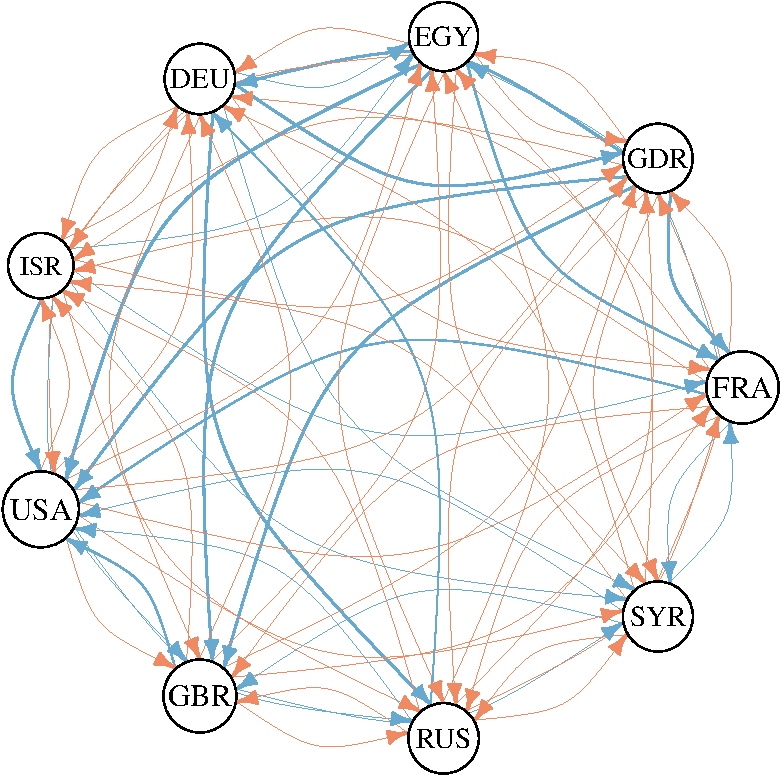
\includegraphics[width=.5\textwidth]{compNet_1972}
		\label{fig:comp72}} & 

	\subfloat[sub1][Compliance: 1992]{
		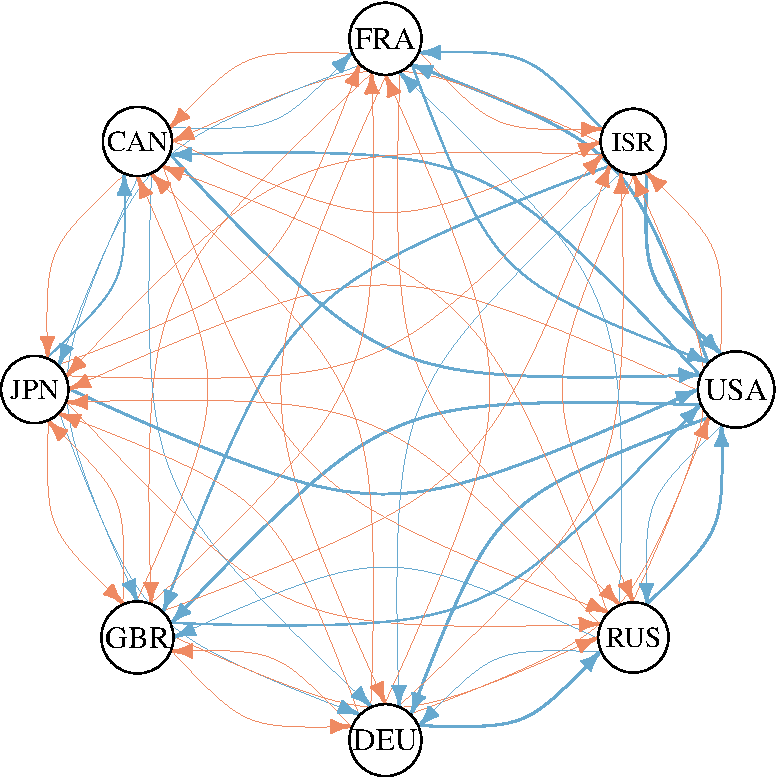
\includegraphics[width=.5\textwidth]{compNet_1992}
		\label{fig:comp92}} \\

	\multicolumn{2}{c}{\subfloat[sub1][Compliance: 2012]{
			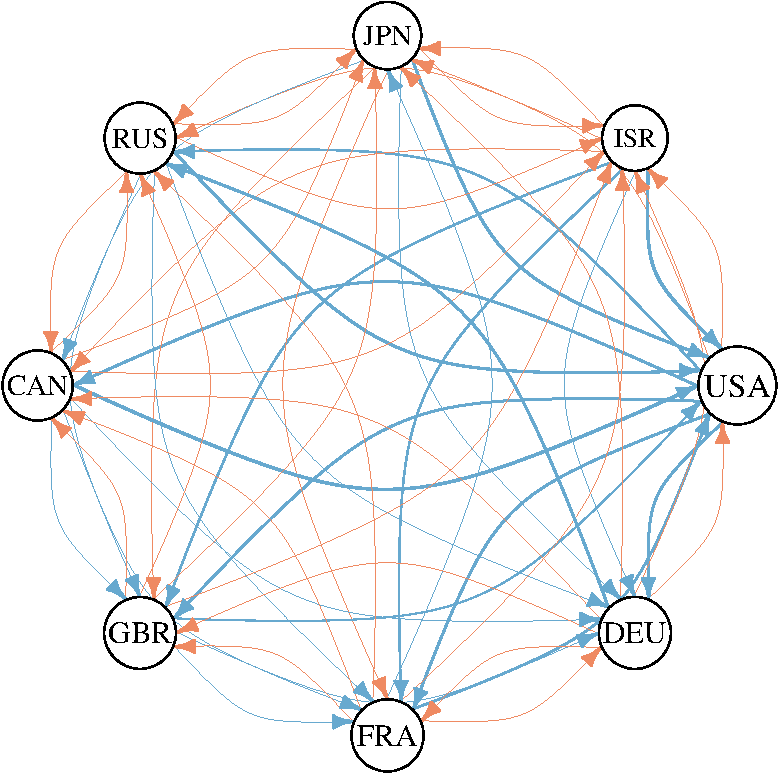
\includegraphics[width=.5\textwidth]{compNet_2012}
			\label{fig:comp02}}}

	% \subfloat[sub1][Sanction: 1972]{
	% 	\includegraphics[width=.33\textwidth]{sancNet_1972}
	% 	\label{fig:sanc72}} & 

	% \subfloat[sub1][Sanction: 1992]{
	% 	\includegraphics[width=.33\textwidth]{sancNet_1992}
	% 	\label{fig:sanc92}} & 

	% \subfloat[sub1][Sanction: 2012]{
	% 	\includegraphics[width=.33\textwidth]{sancNet_2012}
	% 	\label{fig:sanc02}}

	\end{tabular}
	\label{fig:recipNet}
\end{figure}
\FloatBarrier

We extend this intuition to our second key measure, \textit{sanction reciprocity}. Following the same idea as compliance reciprocity, this is a measure of how often a target state has received sanctions from the senders of any given sanction case -- relative to all other sanction interactions of states. The intuition behind this measure is to capture the concept of creating expectations of resolve: states who have been sanctioned multiple times by a sender state are likely to build up a willingness of resistance and not cooperation. This suggests that states receiving sanctions from those with whom they have been sanctioned before are likely to more slowly comply with those states. 

The basic insight is that states whom continually respond to sanctions by sending sanctions of their own are signaling more conflictual rather than cooperative behavior over time. This endogenously formed strategic environment is a dominating factor for the initiation of sanction compliance. Thus, in a world of changing information and strategic incentives, a country will not continue to repetitively comply with a partner state simply out of perceived strategic ties. Countries require continuous signals to build trust and cooperation over time and to maintain a shared understanding of strategic importance to one another. For this reason, we argue that reciprocity is an essential component endogenous to the strategic environment whereby an increase in reciprocity results in an increase in the likelihood of sanction compliance. 

% We are all familiar with the chilling phrase, "a reciprocal exchange of nuclear weapons." Because reciprocity implies returning ill for ill as well as good for good, its moral status is ambiguous. Because it can lead to mutually harmful conflict, its political value may also be questionable. If either of two parties practicing specific reciprocity begins with a malign move, cooperation can never be achieved as long as both persist in this strategy. Axelrod points out that what he calls "echo effects" can produce conflict: "the trouble with TIT FOR TAT is that once a feud gets started, it can continue indefinitely
%%%%%%%%%%%%%%%%%%%%%%

%%%%% Empirics %%%%%
\section*{Data and Analysis}
\label{empirics}

To test the effects of network pressures on sanction compliance we use the Threat and Imposition of Sanctions (TIES) Database developed by \citet{morgan2009threat}. This database includes over 1,400 sanction case threats and initiations from 1945 to 2013. Only sanction cases initiated by 2005 are included but outcomes for cases are recorded until 2013. Our focus here is restricted to sanctions that have actually been imposed rather than simply threatened. Restricting our analysis to sanctions that have been imposed during the period of 1960 to 2005 still leaves us with over 800 unique cases. Our unit of analysis is the case-year, providing us with over 7,500 observations. For each case in the TIES database a final outcome is recorded to describe how and if the case has been resolved. We consider the target of a sanction to have complied, if the target state completely or partially acquiesces to the demands of the sanction senders or negotiates a settlement. This is the same definition of sanction success, which we refer to as compliance, that is employed by \citet{bapat2009multilateral} and \citet{bapat2013determinants}. In using this definition of compliance, approximately 36\% of cases in our dataset end with a state complying by 2013 while another 36\% remain ongoing. The remaining 27\% of cases were terminated for other reasons show below in Table \ref{tab:termCases}. Our focus here is on modeling the time until a target country complies to a sanction using the definition described above. 

\begin{table}[ht]
	\centering
	\begin{tabular}{lc}
		\hline\hline
		Outcome & Frequency \\
		\hline
		Capitulation by Sender After Imposition & 160 \\
		Stalemate after Sanctions Imposition & 71 \\
		\hline\hline
	\end{tabular}
	\caption{Outcomes of sanction cases no longer ongoing where compliance was not achieved.}
	\label{tab:termCases}	
\end{table}

\begin{center}
\textit{Modeling Approach}\\
\end{center}

Next we discuss our modeling approach. To estimate the effect of network pressures on the ability of threatened or sanctioned states to resist compliance, we use Cox proportional hazard (PH) models of the length of threat or sanction periods. Specifically, the dependent variable, sanction spell, is the number of years that a state has not complied to a threat or sanction at time $t$. We model the expected length of sanction spells as a function of a baseline hazard rate and a set of covariates that shift the baseline hazard. The Cox PH specification that we employ is:

\begin{center}
	$\log h_{i}(t | \boldsymbol{X}_{i}) \; = \; h_{0}(t) \times \exp(\boldsymbol{X}_{i} \beta)$,
\end{center}

where the log-hazard rate of compliance in a sanction case, $i$, conditional on having not complied for $t$ years is a function of a common baseline hazard $h_{0}(t)$ and covariates $\boldsymbol{X}$. In employing this approach, we assume no specific functional form for the baseline hazard and instead estimate it non-parametrically from the data.\footnote{To ensure against bias in our parameter estimates we included a vector of case-level shared frailties to account for variations in unit-specific factors. We found similar results with and without the shared frailties, so we report results without the inclusion of this additional term.}  The covariates $\boldsymbol{X}$ operate multiplicatively on the hazard rate, shifting the expected risk of compliance up or down depending on the value of $\beta$.\footnote{\cite{crespo2013political}}

Providing no specific functional form for the baseline hazard necessitates testing the proportional hazard assumption. \citet{keele2010proportionally} notes that not inspecting this assumption in the covariates can lead to severely biased parameter estimates. To address this issue, we first fit smoothing splines for all continuous covariates. After ascertaining that none of the continuous covariates in our model required modeling with splines, we carried out tests of non-proportionality.\footnote{For those covariates where the non-proportional effects assumption does not hold, we include interactions between the covariate and spell duration (log scale).} 

We also impute missing values to avoid excluding instances of compliance. If we employed list-wise deletion, we would lose almost 1,000 country-year observations and 100 unique sanction cases. Previous research has already highlighted how simply deleting missing observations can lead to biased results.\footnote{For example, see \citealp{rubin1976inference,honaker2010missing}.} To impute missing values, we use a copula based approach developed by \citet{hoff:2007}. Details on our imputation process and results based on the original dataset, which are nearly identical, can be found in the \nameref{appendix}.\footnote{We include summary statistics of the original and imputed datasets used for analysis in the \nameref{appendix} as well. } 

In addition to including our two key measures of reciprocity, discussed in the previous section, we control for a variety of other components identified as being important in determining whether a target states complies to a sanction. First, is a simple counter of the number of sender states involved in a sanction to account for the evidence that multilateral sanctions appear to lead to compliance more frequently than unilateral sanctions \citep{bapat2009multilateral}. However, along with many others in the literature, we expect that what determines compliance it is not simply the number of senders involved but also the relationships that a sanctioned state has with senders.

Some of the recent literature on sanction compliance has turned to examining the relationships between the senders and receiver of a sanction. Just as one would imagine that a person is less swayed by the demands of 10 strangers than the demands of a few close friends, we conceptualize senders as most influential when they interact with the target state on a number of dimensions. For example, \cite{mclean2010friends} argue that countries are more likely to comply if they are sanctioned by their major trading partners. To account for these types of explanations, we incorporate a number of variables that describe the relationship a sanctioned state has with its senders. First, we measure the average distance between sender(s) and receiver.\footnote{To construct this measure we use the minimum distance between countries from the Cshapes Dataset \citep{weidmann2010geography}.} Our second covariate relating to proximity is trade, which we measure as the total share of the receiver's trade in that year accounted for by sender states.\footnote{Data for this measure is taken from the Correlates of War (CoW) Trade dataset \citep{barbieri2009trading}.} Last, we measure alliances as the proportion of sender(s) that are allied with the receiver.\footnote{Data for this measure is obtained from the CoW Formal Alliances dataset \citep{gibler2004measuring}.}

Finally, we include a number of covariates to account for domestic explanations of sanction compliance in the extant literature. First is a measure of the target states' domestic institutions from the Polity IV data.\footnote{See \cite{marshall2002polity}. Specifically, we use the ``polity2'' variable from the Polity IV data.} This measure is computed by subtracting a country's autocracy score from its democracy score, and is scaled from 0 to 20. Previous research has shown that sanctions will be more effective when the target states' domestic institutions are more democratic. Second, we control for the level of internal conflict within  a country using the weighted conflict index from the Cross National Time-series Data Archive.\footnote{\cite{banks2011cross}} The expectation in the extant literature is that countries with higher levels of internal instability would be more likely to comply with sanctions. Finally, we use a logged measure of GDP per capita and the percent change in annual GDP, from the World Bank, to account for the argument that economically successful states are better able to weather the pressures of these agreements.

Below we show our full model specification: 

\begin{align*}
		Compliance_{i,t} =& \\
		&Sanction \; Reciprocity_{j,t-1} + Compliance \; Reciprocity_{j,t-1} + \\
		&No. \; Senders_{j} + Distance_{j} + Trade_{j,t-1} + Ally_{j,t-1} + \\
		&Polity_{i,t-1} + Ln(GDP \; Capita)_{i,t-1} +\\
		&GDP \; Growth_{i,t-1} + Internal \; Conflict_{i,t-1} + \epsilon_{i,t}
\end{align*}

where $i$ represents the target of the sanction, $j$ represents the relationship between the set of sender(s) for a particular sanction case and $i$, and $t$ the time period -- variables without a $t$ subscript are time-invariant.

%%%%%%%%%%%%%%%%%%%%%%

%%%%% Empirics %%%%%
\section*{Results}
\label{Results} 

Table~\ref{tab:regResults} displays the results from our model. To contrast with findings from the extant literature, we run the model in three ways. The first column tests the explanations of sanction compliance centered on target state characteristics. In the second column, we add covariates to account for a target's relationships with sender states. The final model incorporates our reciprocity measures. 

% latex table generated in R 3.1.2 by xtable 1.7-4 package
% Sun May 24 13:11:58 2015
\begin{table}[ht]
\centering
{\normalsize
\begin{tabular}{lccc}
 Variable & Model 1 & Model 2 & Model 3 \\ 
  \hline
\hline
Compliance Reciprocity$_{j,t-1}$ &  &  & $0.348^{\ast\ast}$ \\ 
   &  &  & (0.115) \\ 
  Sanction Reciprocity$_{j,t-1}$ &  &  & $-0.15^{\ast\ast}$ \\ 
   &  &  & (0.057) \\ 
   \hline
Number of Senders$_{j,t}$ &  & $0.369^{\ast\ast}$ & $0.356^{\ast\ast}$ \\ 
   &  & (0.086) & (0.086) \\ 
  Distance$_{j,t}$ &  & $1.416^{\ast\ast}$ & $1.426^{\ast\ast}$ \\ 
   &  & (0.28) & (0.284) \\ 
  Trade$_{j,t}$ &  & -1.153 & 3.618 \\ 
   &  & (25.874) & (25.931) \\ 
  Ally$_{j,t}$ &  & 0.05 & 0.09 \\ 
   &  & (0.271) & (0.277) \\ 
   \hline
Polity$_{i,t-1}$ & 0.032 & $0.069^{\ast\ast}$ & $0.067^{\ast\ast}$ \\ 
   & (0.026) & (0.028) & (0.028) \\ 
  Ln(GDP per capita)$_{i,t-1}$ & $-0.331^{\ast\ast}$ & $-0.439^{\ast\ast}$ & $-0.388^{\ast\ast}$ \\ 
   & (0.1) & (0.114) & (0.121) \\ 
  GDP Growth$_{i,t-1}$ & 0.037 & 0.051 & 0.037 \\ 
   & (0.033) & (0.035) & (0.035) \\ 
  Population$_{i,t-1}$ & $-0.197^{\ast\ast}$ & $-0.193^{\ast\ast}$ & -0.142 \\ 
   & (0.083) & (0.096) & (0.1) \\ 
  Internal Conflict$_{i,t-1}$ & 0.001 & 0.003 & 0.002 \\ 
   & (0.025) & (0.025) & (0.025) \\ 
   \hline
n & 3777 & 3764 & 3764 \\ 
  Events & 72 & 72 & 72 \\ 
  Likelihood ratio test & 20.18 (0) & 55.2 (0) & 64.09 (0) \\ 
   \hline
\hline
\end{tabular}
}
\caption{Duration model with time varying covariates estimated using Cox Proportional Hazards. Standard errors in parentheses. $^{**}$ and $^{*}$ indicate significance at $p< 0.05 $ and $p< 0.10 $, respectively.} 
\label{tab:regResults}
\end{table}


We find no support for the argument that high levels of internal stability may prompt a country to comply. Across each specification, we do find that countries with higher levels of GDP per capita take longer to comply with a sanction case, indicating that wealthier countries are able to resist complying to sanctions for lengthier durations. Additionally, like previous work in the literature, when we control for the relationships that a sanctioned state has with its senders, we find that more democratic countries are likely to take a shorter time to comply with sanctions. However, this effect becomes insignificant once we incorporate our network-related covariates. 

Since it is difficult to interpret the substantive meaning of point estimates from the hazard function in Table~\ref{tab:regResults}, we depict Kaplan-Meier estimates of survival probabilities. The y-axis in these charts represents the probability of survival, or in this case the probability that a country will not comply with a sanction, and the x-axis represents time since sanction initiation (measured in years). To depict the substantive effect of our covariates, we set up two scenarios, one in which the value for the covariate of interest is set to its minimum value, depicted in red, and another where it is set to its maximum, depicted in blue. All the other covariates are set to their median. The darker shaded area around the line represents the 90\% confidence interval and the lighter shaded area the 95\% confidence interval. Using these plots, we trace the effect of GDP per capita, in Model 3, on the probability of sanction compliance as a function of time; the results are shown in Figure~\ref{fig:monSurv}. The predicted difference in compliance probabilities between regimes with varying levels of GDP per capita, on the other hand, is quite stark. Just five years after sanction initiation, extremely poor regimes are 15\% more likely to comply than wealthier regimes. 

\begin{figure}[ht]
	\centering
	\caption{Survival probabilities over time by $Ln(GDP \; Capita)_{i,t-1}$. Red designates scenarios in which the covariate is set to its minimum value and blue where it is set to its maximum value. Darker shaded around each line represents the 90\% confidence interval and the lighter shaded area the 95\% confidence interval.}
	% \begin{tabular}{cc}

    % \subfloat[SubFigure 1][Log(GDP per Capita)]{
        \resizebox{.55\textwidth}{!}{% Created by tikzDevice version 0.7.0 on 2015-05-17 07:08:45
% !TEX encoding = UTF-8 Unicode
\begin{tikzpicture}[x=1pt,y=1pt]
\definecolor[named]{fillColor}{rgb}{1.00,1.00,1.00}
\path[use as bounding box,fill=fillColor,fill opacity=0.00] (0,0) rectangle (433.62,289.08);
\begin{scope}
\path[clip] (  0.00,  0.00) rectangle (433.62,289.08);
\definecolor[named]{drawColor}{rgb}{0.00,0.00,0.00}

\path[draw=drawColor,line width= 0.4pt,line join=round,line cap=round] ( 49.20, 61.20) -- (408.42, 61.20);

\path[draw=drawColor,line width= 0.4pt,line join=round,line cap=round] ( 49.20, 61.20) -- ( 49.20, 55.20);

\path[draw=drawColor,line width= 0.4pt,line join=round,line cap=round] (109.07, 61.20) -- (109.07, 55.20);

\path[draw=drawColor,line width= 0.4pt,line join=round,line cap=round] (168.94, 61.20) -- (168.94, 55.20);

\path[draw=drawColor,line width= 0.4pt,line join=round,line cap=round] (228.81, 61.20) -- (228.81, 55.20);

\path[draw=drawColor,line width= 0.4pt,line join=round,line cap=round] (288.68, 61.20) -- (288.68, 55.20);

\path[draw=drawColor,line width= 0.4pt,line join=round,line cap=round] (348.55, 61.20) -- (348.55, 55.20);

\path[draw=drawColor,line width= 0.4pt,line join=round,line cap=round] (408.42, 61.20) -- (408.42, 55.20);

\node[text=drawColor,anchor=base,inner sep=0pt, outer sep=0pt, scale=  1.00] at ( 49.20, 39.60) {0};

\node[text=drawColor,anchor=base,inner sep=0pt, outer sep=0pt, scale=  1.00] at (109.07, 39.60) {5};

\node[text=drawColor,anchor=base,inner sep=0pt, outer sep=0pt, scale=  1.00] at (168.94, 39.60) {10};

\node[text=drawColor,anchor=base,inner sep=0pt, outer sep=0pt, scale=  1.00] at (228.81, 39.60) {15};

\node[text=drawColor,anchor=base,inner sep=0pt, outer sep=0pt, scale=  1.00] at (288.68, 39.60) {20};

\node[text=drawColor,anchor=base,inner sep=0pt, outer sep=0pt, scale=  1.00] at (348.55, 39.60) {25};

\node[text=drawColor,anchor=base,inner sep=0pt, outer sep=0pt, scale=  1.00] at (408.42, 39.60) {30};

\path[draw=drawColor,line width= 0.4pt,line join=round,line cap=round] ( 49.20, 67.82) -- ( 49.20,233.26);

\path[draw=drawColor,line width= 0.4pt,line join=round,line cap=round] ( 49.20, 67.82) -- ( 43.20, 67.82);

\path[draw=drawColor,line width= 0.4pt,line join=round,line cap=round] ( 49.20,100.91) -- ( 43.20,100.91);

\path[draw=drawColor,line width= 0.4pt,line join=round,line cap=round] ( 49.20,134.00) -- ( 43.20,134.00);

\path[draw=drawColor,line width= 0.4pt,line join=round,line cap=round] ( 49.20,167.08) -- ( 43.20,167.08);

\path[draw=drawColor,line width= 0.4pt,line join=round,line cap=round] ( 49.20,200.17) -- ( 43.20,200.17);

\path[draw=drawColor,line width= 0.4pt,line join=round,line cap=round] ( 49.20,233.26) -- ( 43.20,233.26);

\node[text=drawColor,anchor=base east,inner sep=0pt, outer sep=0pt, scale=  1.00] at ( 37.20, 64.37) {0.0};

\node[text=drawColor,anchor=base east,inner sep=0pt, outer sep=0pt, scale=  1.00] at ( 37.20, 97.46) {0.2};

\node[text=drawColor,anchor=base east,inner sep=0pt, outer sep=0pt, scale=  1.00] at ( 37.20,130.55) {0.4};

\node[text=drawColor,anchor=base east,inner sep=0pt, outer sep=0pt, scale=  1.00] at ( 37.20,163.64) {0.6};

\node[text=drawColor,anchor=base east,inner sep=0pt, outer sep=0pt, scale=  1.00] at ( 37.20,196.73) {0.8};

\node[text=drawColor,anchor=base east,inner sep=0pt, outer sep=0pt, scale=  1.00] at ( 37.20,229.82) {1.0};
\end{scope}
\begin{scope}
\path[clip] (  0.00,  0.00) rectangle (433.62,289.08);
\definecolor[named]{drawColor}{rgb}{0.00,0.00,0.00}

\node[text=drawColor,anchor=base,inner sep=0pt, outer sep=0pt, scale=  1.00] at (228.81, 15.60) {Time (Years)};

\node[text=drawColor,rotate= 90.00,anchor=base,inner sep=0pt, outer sep=0pt, scale=  1.00] at ( 10.80,150.54) {Survival Probability};
\end{scope}
\begin{scope}
\path[clip] ( 49.20, 61.20) rectangle (408.42,239.88);
\definecolor[named]{drawColor}{rgb}{0.66,0.66,0.66}

\path[draw=drawColor,line width= 0.4pt,line join=round,line cap=round] ( 49.20,233.26) --
	( 61.17,233.26) --
	( 61.17,210.43) --
	( 73.15,210.43) --
	( 73.15,187.89) --
	( 85.12,187.89) --
	( 85.12,168.12) --
	( 97.10,168.12) --
	( 97.10,158.00) --
	(109.07,158.00) --
	(109.07,154.25) --
	(121.04,154.25) --
	(121.04,152.94) --
	(133.02,152.94) --
	(133.02,151.64) --
	(144.99,151.64) --
	(144.99,150.16) --
	(156.97,150.16) --
	(156.97,148.47) --
	(168.94,148.47) --
	(168.94,146.74) --
	(204.86,146.74) --
	(204.86,144.03) --
	(216.84,144.03) --
	(216.84,140.24) --
	(264.73,140.24) --
	(264.73,131.70) --
	(288.68,131.70) --
	(288.68,122.18) --
	(300.65,122.18) --
	(300.65,113.89) --
	(336.58,113.89) --
	(336.58,106.87) --
	(433.62,106.87);

\path[draw=drawColor,line width= 0.4pt,line join=round,line cap=round] ( 57.99,210.43) -- ( 64.36,210.43);

\path[draw=drawColor,line width= 0.4pt,line join=round,line cap=round] ( 61.17,207.25) -- ( 61.17,213.61);

\path[draw=drawColor,line width= 0.4pt,line join=round,line cap=round] ( 69.97,187.89) -- ( 76.33,187.89);

\path[draw=drawColor,line width= 0.4pt,line join=round,line cap=round] ( 73.15,184.71) -- ( 73.15,191.07);

\path[draw=drawColor,line width= 0.4pt,line join=round,line cap=round] ( 81.94,168.12) -- ( 88.30,168.12);

\path[draw=drawColor,line width= 0.4pt,line join=round,line cap=round] ( 85.12,164.94) -- ( 85.12,171.30);

\path[draw=drawColor,line width= 0.4pt,line join=round,line cap=round] ( 93.91,158.00) -- (100.28,158.00);

\path[draw=drawColor,line width= 0.4pt,line join=round,line cap=round] ( 97.10,154.82) -- ( 97.10,161.18);

\path[draw=drawColor,line width= 0.4pt,line join=round,line cap=round] (105.89,154.25) -- (112.25,154.25);

\path[draw=drawColor,line width= 0.4pt,line join=round,line cap=round] (109.07,151.07) -- (109.07,157.43);

\path[draw=drawColor,line width= 0.4pt,line join=round,line cap=round] (117.86,152.94) -- (124.23,152.94);

\path[draw=drawColor,line width= 0.4pt,line join=round,line cap=round] (121.04,149.76) -- (121.04,156.12);

\path[draw=drawColor,line width= 0.4pt,line join=round,line cap=round] (129.84,151.64) -- (136.20,151.64);

\path[draw=drawColor,line width= 0.4pt,line join=round,line cap=round] (133.02,148.46) -- (133.02,154.82);

\path[draw=drawColor,line width= 0.4pt,line join=round,line cap=round] (141.81,150.16) -- (148.17,150.16);

\path[draw=drawColor,line width= 0.4pt,line join=round,line cap=round] (144.99,146.97) -- (144.99,153.34);

\path[draw=drawColor,line width= 0.4pt,line join=round,line cap=round] (153.78,148.47) -- (160.15,148.47);

\path[draw=drawColor,line width= 0.4pt,line join=round,line cap=round] (156.97,145.28) -- (156.97,151.65);

\path[draw=drawColor,line width= 0.4pt,line join=round,line cap=round] (165.76,146.74) -- (172.12,146.74);

\path[draw=drawColor,line width= 0.4pt,line join=round,line cap=round] (168.94,143.56) -- (168.94,149.92);

\path[draw=drawColor,line width= 0.4pt,line join=round,line cap=round] (177.73,146.74) -- (184.10,146.74);

\path[draw=drawColor,line width= 0.4pt,line join=round,line cap=round] (180.91,143.56) -- (180.91,149.92);

\path[draw=drawColor,line width= 0.4pt,line join=round,line cap=round] (189.71,146.74) -- (196.07,146.74);

\path[draw=drawColor,line width= 0.4pt,line join=round,line cap=round] (192.89,143.56) -- (192.89,149.92);

\path[draw=drawColor,line width= 0.4pt,line join=round,line cap=round] (201.68,144.03) -- (208.04,144.03);

\path[draw=drawColor,line width= 0.4pt,line join=round,line cap=round] (204.86,140.85) -- (204.86,147.22);

\path[draw=drawColor,line width= 0.4pt,line join=round,line cap=round] (213.65,140.24) -- (220.02,140.24);

\path[draw=drawColor,line width= 0.4pt,line join=round,line cap=round] (216.84,137.06) -- (216.84,143.43);

\path[draw=drawColor,line width= 0.4pt,line join=round,line cap=round] (225.63,140.24) -- (231.99,140.24);

\path[draw=drawColor,line width= 0.4pt,line join=round,line cap=round] (228.81,137.06) -- (228.81,143.43);

\path[draw=drawColor,line width= 0.4pt,line join=round,line cap=round] (237.60,140.24) -- (243.97,140.24);

\path[draw=drawColor,line width= 0.4pt,line join=round,line cap=round] (240.78,137.06) -- (240.78,143.43);

\path[draw=drawColor,line width= 0.4pt,line join=round,line cap=round] (249.58,140.24) -- (255.94,140.24);

\path[draw=drawColor,line width= 0.4pt,line join=round,line cap=round] (252.76,137.06) -- (252.76,143.43);

\path[draw=drawColor,line width= 0.4pt,line join=round,line cap=round] (261.55,131.70) -- (267.91,131.70);

\path[draw=drawColor,line width= 0.4pt,line join=round,line cap=round] (264.73,128.52) -- (264.73,134.88);

\path[draw=drawColor,line width= 0.4pt,line join=round,line cap=round] (273.52,131.70) -- (279.89,131.70);

\path[draw=drawColor,line width= 0.4pt,line join=round,line cap=round] (276.71,128.52) -- (276.71,134.88);

\path[draw=drawColor,line width= 0.4pt,line join=round,line cap=round] (285.50,122.18) -- (291.86,122.18);

\path[draw=drawColor,line width= 0.4pt,line join=round,line cap=round] (288.68,119.00) -- (288.68,125.37);

\path[draw=drawColor,line width= 0.4pt,line join=round,line cap=round] (297.47,113.89) -- (303.84,113.89);

\path[draw=drawColor,line width= 0.4pt,line join=round,line cap=round] (300.65,110.71) -- (300.65,117.08);

\path[draw=drawColor,line width= 0.4pt,line join=round,line cap=round] (309.45,113.89) -- (315.81,113.89);

\path[draw=drawColor,line width= 0.4pt,line join=round,line cap=round] (312.63,110.71) -- (312.63,117.08);

\path[draw=drawColor,line width= 0.4pt,line join=round,line cap=round] (321.42,113.89) -- (327.78,113.89);

\path[draw=drawColor,line width= 0.4pt,line join=round,line cap=round] (324.60,110.71) -- (324.60,117.08);

\path[draw=drawColor,line width= 0.4pt,line join=round,line cap=round] (333.39,106.87) -- (339.76,106.87);

\path[draw=drawColor,line width= 0.4pt,line join=round,line cap=round] (336.58,103.69) -- (336.58,110.05);

\path[draw=drawColor,line width= 0.4pt,line join=round,line cap=round] (345.37,106.87) -- (351.73,106.87);

\path[draw=drawColor,line width= 0.4pt,line join=round,line cap=round] (348.55,103.69) -- (348.55,110.05);

\path[draw=drawColor,line width= 0.4pt,line join=round,line cap=round] (357.34,106.87) -- (363.71,106.87);

\path[draw=drawColor,line width= 0.4pt,line join=round,line cap=round] (360.52,103.69) -- (360.52,110.05);

\path[draw=drawColor,line width= 0.4pt,line join=round,line cap=round] (369.32,106.87) -- (375.68,106.87);

\path[draw=drawColor,line width= 0.4pt,line join=round,line cap=round] (372.50,103.69) -- (372.50,110.05);

\path[draw=drawColor,line width= 0.4pt,line join=round,line cap=round] (381.29,106.87) -- (387.65,106.87);

\path[draw=drawColor,line width= 0.4pt,line join=round,line cap=round] (384.47,103.69) -- (384.47,110.05);

\path[draw=drawColor,line width= 0.4pt,line join=round,line cap=round] (393.26,106.87) -- (399.63,106.87);

\path[draw=drawColor,line width= 0.4pt,line join=round,line cap=round] (396.45,103.69) -- (396.45,110.05);

\path[draw=drawColor,line width= 0.4pt,line join=round,line cap=round] (405.24,106.87) -- (411.60,106.87);

\path[draw=drawColor,line width= 0.4pt,line join=round,line cap=round] (408.42,103.69) -- (408.42,110.05);

\path[draw=drawColor,line width= 0.4pt,line join=round,line cap=round] (417.21,106.87) -- (423.58,106.87);

\path[draw=drawColor,line width= 0.4pt,line join=round,line cap=round] (420.39,103.69) -- (420.39,110.05);

\path[draw=drawColor,line width= 0.4pt,line join=round,line cap=round] (429.19,106.87) -- (433.62,106.87);

\path[draw=drawColor,line width= 0.4pt,line join=round,line cap=round] (432.37,103.69) -- (432.37,110.05);
\definecolor[named]{drawColor}{rgb}{0.00,0.00,0.00}

\path[draw=drawColor,line width= 0.4pt,line join=round,line cap=round] ( 49.20,233.26) --
	( 61.17,233.26) --
	( 61.17,231.33) --
	( 73.15,231.33) --
	( 73.15,229.11) --
	( 85.12,229.11) --
	( 85.12,226.83) --
	( 97.10,226.83) --
	( 97.10,225.50) --
	(109.07,225.50) --
	(109.07,224.97) --
	(121.04,224.97) --
	(121.04,224.78) --
	(133.02,224.78) --
	(133.02,224.59) --
	(144.99,224.59) --
	(144.99,224.36) --
	(156.97,224.36) --
	(156.97,224.11) --
	(168.94,224.11) --
	(168.94,223.84) --
	(204.86,223.84) --
	(204.86,223.41) --
	(216.84,223.41) --
	(216.84,222.78) --
	(264.73,222.78) --
	(264.73,221.25) --
	(288.68,221.25) --
	(288.68,219.30) --
	(300.65,219.30) --
	(300.65,217.33) --
	(336.58,217.33) --
	(336.58,215.38) --
	(433.62,215.38);

\path[draw=drawColor,line width= 0.4pt,line join=round,line cap=round] ( 57.99,231.33) -- ( 64.36,231.33);

\path[draw=drawColor,line width= 0.4pt,line join=round,line cap=round] ( 61.17,228.15) -- ( 61.17,234.51);

\path[draw=drawColor,line width= 0.4pt,line join=round,line cap=round] ( 69.97,229.11) -- ( 76.33,229.11);

\path[draw=drawColor,line width= 0.4pt,line join=round,line cap=round] ( 73.15,225.93) -- ( 73.15,232.30);

\path[draw=drawColor,line width= 0.4pt,line join=round,line cap=round] ( 81.94,226.83) -- ( 88.30,226.83);

\path[draw=drawColor,line width= 0.4pt,line join=round,line cap=round] ( 85.12,223.65) -- ( 85.12,230.01);

\path[draw=drawColor,line width= 0.4pt,line join=round,line cap=round] ( 93.91,225.50) -- (100.28,225.50);

\path[draw=drawColor,line width= 0.4pt,line join=round,line cap=round] ( 97.10,222.31) -- ( 97.10,228.68);

\path[draw=drawColor,line width= 0.4pt,line join=round,line cap=round] (105.89,224.97) -- (112.25,224.97);

\path[draw=drawColor,line width= 0.4pt,line join=round,line cap=round] (109.07,221.78) -- (109.07,228.15);

\path[draw=drawColor,line width= 0.4pt,line join=round,line cap=round] (117.86,224.78) -- (124.23,224.78);

\path[draw=drawColor,line width= 0.4pt,line join=round,line cap=round] (121.04,221.59) -- (121.04,227.96);

\path[draw=drawColor,line width= 0.4pt,line join=round,line cap=round] (129.84,224.59) -- (136.20,224.59);

\path[draw=drawColor,line width= 0.4pt,line join=round,line cap=round] (133.02,221.40) -- (133.02,227.77);

\path[draw=drawColor,line width= 0.4pt,line join=round,line cap=round] (141.81,224.36) -- (148.17,224.36);

\path[draw=drawColor,line width= 0.4pt,line join=round,line cap=round] (144.99,221.18) -- (144.99,227.55);

\path[draw=drawColor,line width= 0.4pt,line join=round,line cap=round] (153.78,224.11) -- (160.15,224.11);

\path[draw=drawColor,line width= 0.4pt,line join=round,line cap=round] (156.97,220.93) -- (156.97,227.29);

\path[draw=drawColor,line width= 0.4pt,line join=round,line cap=round] (165.76,223.84) -- (172.12,223.84);

\path[draw=drawColor,line width= 0.4pt,line join=round,line cap=round] (168.94,220.66) -- (168.94,227.02);

\path[draw=drawColor,line width= 0.4pt,line join=round,line cap=round] (177.73,223.84) -- (184.10,223.84);

\path[draw=drawColor,line width= 0.4pt,line join=round,line cap=round] (180.91,220.66) -- (180.91,227.02);

\path[draw=drawColor,line width= 0.4pt,line join=round,line cap=round] (189.71,223.84) -- (196.07,223.84);

\path[draw=drawColor,line width= 0.4pt,line join=round,line cap=round] (192.89,220.66) -- (192.89,227.02);

\path[draw=drawColor,line width= 0.4pt,line join=round,line cap=round] (201.68,223.41) -- (208.04,223.41);

\path[draw=drawColor,line width= 0.4pt,line join=round,line cap=round] (204.86,220.23) -- (204.86,226.59);

\path[draw=drawColor,line width= 0.4pt,line join=round,line cap=round] (213.65,222.78) -- (220.02,222.78);

\path[draw=drawColor,line width= 0.4pt,line join=round,line cap=round] (216.84,219.60) -- (216.84,225.96);

\path[draw=drawColor,line width= 0.4pt,line join=round,line cap=round] (225.63,222.78) -- (231.99,222.78);

\path[draw=drawColor,line width= 0.4pt,line join=round,line cap=round] (228.81,219.60) -- (228.81,225.96);

\path[draw=drawColor,line width= 0.4pt,line join=round,line cap=round] (237.60,222.78) -- (243.97,222.78);

\path[draw=drawColor,line width= 0.4pt,line join=round,line cap=round] (240.78,219.60) -- (240.78,225.96);

\path[draw=drawColor,line width= 0.4pt,line join=round,line cap=round] (249.58,222.78) -- (255.94,222.78);

\path[draw=drawColor,line width= 0.4pt,line join=round,line cap=round] (252.76,219.60) -- (252.76,225.96);

\path[draw=drawColor,line width= 0.4pt,line join=round,line cap=round] (261.55,221.25) -- (267.91,221.25);

\path[draw=drawColor,line width= 0.4pt,line join=round,line cap=round] (264.73,218.07) -- (264.73,224.43);

\path[draw=drawColor,line width= 0.4pt,line join=round,line cap=round] (273.52,221.25) -- (279.89,221.25);

\path[draw=drawColor,line width= 0.4pt,line join=round,line cap=round] (276.71,218.07) -- (276.71,224.43);

\path[draw=drawColor,line width= 0.4pt,line join=round,line cap=round] (285.50,219.30) -- (291.86,219.30);

\path[draw=drawColor,line width= 0.4pt,line join=round,line cap=round] (288.68,216.12) -- (288.68,222.48);

\path[draw=drawColor,line width= 0.4pt,line join=round,line cap=round] (297.47,217.33) -- (303.84,217.33);

\path[draw=drawColor,line width= 0.4pt,line join=round,line cap=round] (300.65,214.15) -- (300.65,220.51);

\path[draw=drawColor,line width= 0.4pt,line join=round,line cap=round] (309.45,217.33) -- (315.81,217.33);

\path[draw=drawColor,line width= 0.4pt,line join=round,line cap=round] (312.63,214.15) -- (312.63,220.51);

\path[draw=drawColor,line width= 0.4pt,line join=round,line cap=round] (321.42,217.33) -- (327.78,217.33);

\path[draw=drawColor,line width= 0.4pt,line join=round,line cap=round] (324.60,214.15) -- (324.60,220.51);

\path[draw=drawColor,line width= 0.4pt,line join=round,line cap=round] (333.39,215.38) -- (339.76,215.38);

\path[draw=drawColor,line width= 0.4pt,line join=round,line cap=round] (336.58,212.20) -- (336.58,218.56);

\path[draw=drawColor,line width= 0.4pt,line join=round,line cap=round] (345.37,215.38) -- (351.73,215.38);

\path[draw=drawColor,line width= 0.4pt,line join=round,line cap=round] (348.55,212.20) -- (348.55,218.56);

\path[draw=drawColor,line width= 0.4pt,line join=round,line cap=round] (357.34,215.38) -- (363.71,215.38);

\path[draw=drawColor,line width= 0.4pt,line join=round,line cap=round] (360.52,212.20) -- (360.52,218.56);

\path[draw=drawColor,line width= 0.4pt,line join=round,line cap=round] (369.32,215.38) -- (375.68,215.38);

\path[draw=drawColor,line width= 0.4pt,line join=round,line cap=round] (372.50,212.20) -- (372.50,218.56);

\path[draw=drawColor,line width= 0.4pt,line join=round,line cap=round] (381.29,215.38) -- (387.65,215.38);

\path[draw=drawColor,line width= 0.4pt,line join=round,line cap=round] (384.47,212.20) -- (384.47,218.56);

\path[draw=drawColor,line width= 0.4pt,line join=round,line cap=round] (393.26,215.38) -- (399.63,215.38);

\path[draw=drawColor,line width= 0.4pt,line join=round,line cap=round] (396.45,212.20) -- (396.45,218.56);

\path[draw=drawColor,line width= 0.4pt,line join=round,line cap=round] (405.24,215.38) -- (411.60,215.38);

\path[draw=drawColor,line width= 0.4pt,line join=round,line cap=round] (408.42,212.20) -- (408.42,218.56);

\path[draw=drawColor,line width= 0.4pt,line join=round,line cap=round] (417.21,215.38) -- (423.58,215.38);

\path[draw=drawColor,line width= 0.4pt,line join=round,line cap=round] (420.39,212.20) -- (420.39,218.56);

\path[draw=drawColor,line width= 0.4pt,line join=round,line cap=round] (429.19,215.38) -- (433.62,215.38);

\path[draw=drawColor,line width= 0.4pt,line join=round,line cap=round] (432.37,212.20) -- (432.37,218.56);
\end{scope}
\end{tikzpicture}
}	
        % \label{fig:gdpSurv}}

	% \subfloat[SubFigure 2][Polity]{
	% 	\resizebox{.45\textwidth}{!}{% Created by tikzDevice version 0.7.0 on 2015-05-17 07:08:44
% !TEX encoding = UTF-8 Unicode
\begin{tikzpicture}[x=1pt,y=1pt]
\definecolor[named]{fillColor}{rgb}{1.00,1.00,1.00}
\path[use as bounding box,fill=fillColor,fill opacity=0.00] (0,0) rectangle (433.62,289.08);
\begin{scope}
\path[clip] (  0.00,  0.00) rectangle (433.62,289.08);
\definecolor[named]{drawColor}{rgb}{0.00,0.00,0.00}

\path[draw=drawColor,line width= 0.4pt,line join=round,line cap=round] ( 49.20, 61.20) -- (408.42, 61.20);

\path[draw=drawColor,line width= 0.4pt,line join=round,line cap=round] ( 49.20, 61.20) -- ( 49.20, 55.20);

\path[draw=drawColor,line width= 0.4pt,line join=round,line cap=round] (109.07, 61.20) -- (109.07, 55.20);

\path[draw=drawColor,line width= 0.4pt,line join=round,line cap=round] (168.94, 61.20) -- (168.94, 55.20);

\path[draw=drawColor,line width= 0.4pt,line join=round,line cap=round] (228.81, 61.20) -- (228.81, 55.20);

\path[draw=drawColor,line width= 0.4pt,line join=round,line cap=round] (288.68, 61.20) -- (288.68, 55.20);

\path[draw=drawColor,line width= 0.4pt,line join=round,line cap=round] (348.55, 61.20) -- (348.55, 55.20);

\path[draw=drawColor,line width= 0.4pt,line join=round,line cap=round] (408.42, 61.20) -- (408.42, 55.20);

\node[text=drawColor,anchor=base,inner sep=0pt, outer sep=0pt, scale=  1.00] at ( 49.20, 39.60) {0};

\node[text=drawColor,anchor=base,inner sep=0pt, outer sep=0pt, scale=  1.00] at (109.07, 39.60) {5};

\node[text=drawColor,anchor=base,inner sep=0pt, outer sep=0pt, scale=  1.00] at (168.94, 39.60) {10};

\node[text=drawColor,anchor=base,inner sep=0pt, outer sep=0pt, scale=  1.00] at (228.81, 39.60) {15};

\node[text=drawColor,anchor=base,inner sep=0pt, outer sep=0pt, scale=  1.00] at (288.68, 39.60) {20};

\node[text=drawColor,anchor=base,inner sep=0pt, outer sep=0pt, scale=  1.00] at (348.55, 39.60) {25};

\node[text=drawColor,anchor=base,inner sep=0pt, outer sep=0pt, scale=  1.00] at (408.42, 39.60) {30};

\path[draw=drawColor,line width= 0.4pt,line join=round,line cap=round] ( 49.20, 67.82) -- ( 49.20,233.26);

\path[draw=drawColor,line width= 0.4pt,line join=round,line cap=round] ( 49.20, 67.82) -- ( 43.20, 67.82);

\path[draw=drawColor,line width= 0.4pt,line join=round,line cap=round] ( 49.20,100.91) -- ( 43.20,100.91);

\path[draw=drawColor,line width= 0.4pt,line join=round,line cap=round] ( 49.20,134.00) -- ( 43.20,134.00);

\path[draw=drawColor,line width= 0.4pt,line join=round,line cap=round] ( 49.20,167.08) -- ( 43.20,167.08);

\path[draw=drawColor,line width= 0.4pt,line join=round,line cap=round] ( 49.20,200.17) -- ( 43.20,200.17);

\path[draw=drawColor,line width= 0.4pt,line join=round,line cap=round] ( 49.20,233.26) -- ( 43.20,233.26);

\node[text=drawColor,anchor=base east,inner sep=0pt, outer sep=0pt, scale=  1.00] at ( 37.20, 64.37) {0.0};

\node[text=drawColor,anchor=base east,inner sep=0pt, outer sep=0pt, scale=  1.00] at ( 37.20, 97.46) {0.2};

\node[text=drawColor,anchor=base east,inner sep=0pt, outer sep=0pt, scale=  1.00] at ( 37.20,130.55) {0.4};

\node[text=drawColor,anchor=base east,inner sep=0pt, outer sep=0pt, scale=  1.00] at ( 37.20,163.64) {0.6};

\node[text=drawColor,anchor=base east,inner sep=0pt, outer sep=0pt, scale=  1.00] at ( 37.20,196.73) {0.8};

\node[text=drawColor,anchor=base east,inner sep=0pt, outer sep=0pt, scale=  1.00] at ( 37.20,229.82) {1.0};
\end{scope}
\begin{scope}
\path[clip] (  0.00,  0.00) rectangle (433.62,289.08);
\definecolor[named]{drawColor}{rgb}{0.00,0.00,0.00}

\node[text=drawColor,anchor=base,inner sep=0pt, outer sep=0pt, scale=  1.00] at (228.81, 15.60) {Time (Years)};

\node[text=drawColor,rotate= 90.00,anchor=base,inner sep=0pt, outer sep=0pt, scale=  1.00] at ( 10.80,150.54) {Survival Probability};
\end{scope}
\begin{scope}
\path[clip] ( 49.20, 61.20) rectangle (408.42,239.88);
\definecolor[named]{drawColor}{rgb}{0.66,0.66,0.66}

\path[draw=drawColor,line width= 0.4pt,line join=round,line cap=round] ( 49.20,233.26) --
	( 61.17,233.26) --
	( 61.17,231.75) --
	( 73.15,231.75) --
	( 73.15,230.01) --
	( 85.12,230.01) --
	( 85.12,228.21) --
	( 97.10,228.21) --
	( 97.10,227.16) --
	(109.07,227.16) --
	(109.07,226.74) --
	(121.04,226.74) --
	(121.04,226.59) --
	(133.02,226.59) --
	(133.02,226.44) --
	(144.99,226.44) --
	(144.99,226.27) --
	(156.97,226.27) --
	(156.97,226.06) --
	(168.94,226.06) --
	(168.94,225.85) --
	(204.86,225.85) --
	(204.86,225.51) --
	(216.84,225.51) --
	(216.84,225.01) --
	(264.73,225.01) --
	(264.73,223.79) --
	(288.68,223.79) --
	(288.68,222.24) --
	(300.65,222.24) --
	(300.65,220.67) --
	(336.58,220.67) --
	(336.58,219.11) --
	(433.62,219.11);

\path[draw=drawColor,line width= 0.4pt,line join=round,line cap=round] ( 57.99,231.75) -- ( 64.36,231.75);

\path[draw=drawColor,line width= 0.4pt,line join=round,line cap=round] ( 61.17,228.57) -- ( 61.17,234.93);

\path[draw=drawColor,line width= 0.4pt,line join=round,line cap=round] ( 69.97,230.01) -- ( 76.33,230.01);

\path[draw=drawColor,line width= 0.4pt,line join=round,line cap=round] ( 73.15,226.83) -- ( 73.15,233.19);

\path[draw=drawColor,line width= 0.4pt,line join=round,line cap=round] ( 81.94,228.21) -- ( 88.30,228.21);

\path[draw=drawColor,line width= 0.4pt,line join=round,line cap=round] ( 85.12,225.03) -- ( 85.12,231.40);

\path[draw=drawColor,line width= 0.4pt,line join=round,line cap=round] ( 93.91,227.16) -- (100.28,227.16);

\path[draw=drawColor,line width= 0.4pt,line join=round,line cap=round] ( 97.10,223.98) -- ( 97.10,230.34);

\path[draw=drawColor,line width= 0.4pt,line join=round,line cap=round] (105.89,226.74) -- (112.25,226.74);

\path[draw=drawColor,line width= 0.4pt,line join=round,line cap=round] (109.07,223.56) -- (109.07,229.92);

\path[draw=drawColor,line width= 0.4pt,line join=round,line cap=round] (117.86,226.59) -- (124.23,226.59);

\path[draw=drawColor,line width= 0.4pt,line join=round,line cap=round] (121.04,223.41) -- (121.04,229.77);

\path[draw=drawColor,line width= 0.4pt,line join=round,line cap=round] (129.84,226.44) -- (136.20,226.44);

\path[draw=drawColor,line width= 0.4pt,line join=round,line cap=round] (133.02,223.26) -- (133.02,229.62);

\path[draw=drawColor,line width= 0.4pt,line join=round,line cap=round] (141.81,226.27) -- (148.17,226.27);

\path[draw=drawColor,line width= 0.4pt,line join=round,line cap=round] (144.99,223.08) -- (144.99,229.45);

\path[draw=drawColor,line width= 0.4pt,line join=round,line cap=round] (153.78,226.06) -- (160.15,226.06);

\path[draw=drawColor,line width= 0.4pt,line join=round,line cap=round] (156.97,222.88) -- (156.97,229.24);

\path[draw=drawColor,line width= 0.4pt,line join=round,line cap=round] (165.76,225.85) -- (172.12,225.85);

\path[draw=drawColor,line width= 0.4pt,line join=round,line cap=round] (168.94,222.67) -- (168.94,229.03);

\path[draw=drawColor,line width= 0.4pt,line join=round,line cap=round] (177.73,225.85) -- (184.10,225.85);

\path[draw=drawColor,line width= 0.4pt,line join=round,line cap=round] (180.91,222.67) -- (180.91,229.03);

\path[draw=drawColor,line width= 0.4pt,line join=round,line cap=round] (189.71,225.85) -- (196.07,225.85);

\path[draw=drawColor,line width= 0.4pt,line join=round,line cap=round] (192.89,222.67) -- (192.89,229.03);

\path[draw=drawColor,line width= 0.4pt,line join=round,line cap=round] (201.68,225.51) -- (208.04,225.51);

\path[draw=drawColor,line width= 0.4pt,line join=round,line cap=round] (204.86,222.33) -- (204.86,228.69);

\path[draw=drawColor,line width= 0.4pt,line join=round,line cap=round] (213.65,225.01) -- (220.02,225.01);

\path[draw=drawColor,line width= 0.4pt,line join=round,line cap=round] (216.84,221.83) -- (216.84,228.19);

\path[draw=drawColor,line width= 0.4pt,line join=round,line cap=round] (225.63,225.01) -- (231.99,225.01);

\path[draw=drawColor,line width= 0.4pt,line join=round,line cap=round] (228.81,221.83) -- (228.81,228.19);

\path[draw=drawColor,line width= 0.4pt,line join=round,line cap=round] (237.60,225.01) -- (243.97,225.01);

\path[draw=drawColor,line width= 0.4pt,line join=round,line cap=round] (240.78,221.83) -- (240.78,228.19);

\path[draw=drawColor,line width= 0.4pt,line join=round,line cap=round] (249.58,225.01) -- (255.94,225.01);

\path[draw=drawColor,line width= 0.4pt,line join=round,line cap=round] (252.76,221.83) -- (252.76,228.19);

\path[draw=drawColor,line width= 0.4pt,line join=round,line cap=round] (261.55,223.79) -- (267.91,223.79);

\path[draw=drawColor,line width= 0.4pt,line join=round,line cap=round] (264.73,220.61) -- (264.73,226.98);

\path[draw=drawColor,line width= 0.4pt,line join=round,line cap=round] (273.52,223.79) -- (279.89,223.79);

\path[draw=drawColor,line width= 0.4pt,line join=round,line cap=round] (276.71,220.61) -- (276.71,226.98);

\path[draw=drawColor,line width= 0.4pt,line join=round,line cap=round] (285.50,222.24) -- (291.86,222.24);

\path[draw=drawColor,line width= 0.4pt,line join=round,line cap=round] (288.68,219.06) -- (288.68,225.43);

\path[draw=drawColor,line width= 0.4pt,line join=round,line cap=round] (297.47,220.67) -- (303.84,220.67);

\path[draw=drawColor,line width= 0.4pt,line join=round,line cap=round] (300.65,217.49) -- (300.65,223.85);

\path[draw=drawColor,line width= 0.4pt,line join=round,line cap=round] (309.45,220.67) -- (315.81,220.67);

\path[draw=drawColor,line width= 0.4pt,line join=round,line cap=round] (312.63,217.49) -- (312.63,223.85);

\path[draw=drawColor,line width= 0.4pt,line join=round,line cap=round] (321.42,220.67) -- (327.78,220.67);

\path[draw=drawColor,line width= 0.4pt,line join=round,line cap=round] (324.60,217.49) -- (324.60,223.85);

\path[draw=drawColor,line width= 0.4pt,line join=round,line cap=round] (333.39,219.11) -- (339.76,219.11);

\path[draw=drawColor,line width= 0.4pt,line join=round,line cap=round] (336.58,215.93) -- (336.58,222.29);

\path[draw=drawColor,line width= 0.4pt,line join=round,line cap=round] (345.37,219.11) -- (351.73,219.11);

\path[draw=drawColor,line width= 0.4pt,line join=round,line cap=round] (348.55,215.93) -- (348.55,222.29);

\path[draw=drawColor,line width= 0.4pt,line join=round,line cap=round] (357.34,219.11) -- (363.71,219.11);

\path[draw=drawColor,line width= 0.4pt,line join=round,line cap=round] (360.52,215.93) -- (360.52,222.29);

\path[draw=drawColor,line width= 0.4pt,line join=round,line cap=round] (369.32,219.11) -- (375.68,219.11);

\path[draw=drawColor,line width= 0.4pt,line join=round,line cap=round] (372.50,215.93) -- (372.50,222.29);

\path[draw=drawColor,line width= 0.4pt,line join=round,line cap=round] (381.29,219.11) -- (387.65,219.11);

\path[draw=drawColor,line width= 0.4pt,line join=round,line cap=round] (384.47,215.93) -- (384.47,222.29);

\path[draw=drawColor,line width= 0.4pt,line join=round,line cap=round] (393.26,219.11) -- (399.63,219.11);

\path[draw=drawColor,line width= 0.4pt,line join=round,line cap=round] (396.45,215.93) -- (396.45,222.29);

\path[draw=drawColor,line width= 0.4pt,line join=round,line cap=round] (405.24,219.11) -- (411.60,219.11);

\path[draw=drawColor,line width= 0.4pt,line join=round,line cap=round] (408.42,215.93) -- (408.42,222.29);

\path[draw=drawColor,line width= 0.4pt,line join=round,line cap=round] (417.21,219.11) -- (423.58,219.11);

\path[draw=drawColor,line width= 0.4pt,line join=round,line cap=round] (420.39,215.93) -- (420.39,222.29);

\path[draw=drawColor,line width= 0.4pt,line join=round,line cap=round] (429.19,219.11) -- (433.62,219.11);

\path[draw=drawColor,line width= 0.4pt,line join=round,line cap=round] (432.37,215.93) -- (432.37,222.29);
\definecolor[named]{drawColor}{rgb}{0.00,0.00,0.00}

\path[draw=drawColor,line width= 0.4pt,line join=round,line cap=round] ( 49.20,233.26) --
	( 61.17,233.26) --
	( 61.17,227.94) --
	( 73.15,227.94) --
	( 73.15,221.99) --
	( 85.12,221.99) --
	( 85.12,216.01) --
	( 97.10,216.01) --
	( 97.10,212.58) --
	(109.07,212.58) --
	(109.07,211.23) --
	(121.04,211.23) --
	(121.04,210.75) --
	(133.02,210.75) --
	(133.02,210.27) --
	(144.99,210.27) --
	(144.99,209.71) --
	(156.97,209.71) --
	(156.97,209.06) --
	(168.94,209.06) --
	(168.94,208.39) --
	(204.86,208.39) --
	(204.86,207.32) --
	(216.84,207.32) --
	(216.84,205.76) --
	(264.73,205.76) --
	(264.73,202.00) --
	(288.68,202.00) --
	(288.68,197.32) --
	(300.65,197.32) --
	(300.65,192.69) --
	(336.58,192.69) --
	(336.58,188.23) --
	(433.62,188.23);

\path[draw=drawColor,line width= 0.4pt,line join=round,line cap=round] ( 57.99,227.94) -- ( 64.36,227.94);

\path[draw=drawColor,line width= 0.4pt,line join=round,line cap=round] ( 61.17,224.76) -- ( 61.17,231.12);

\path[draw=drawColor,line width= 0.4pt,line join=round,line cap=round] ( 69.97,221.99) -- ( 76.33,221.99);

\path[draw=drawColor,line width= 0.4pt,line join=round,line cap=round] ( 73.15,218.81) -- ( 73.15,225.17);

\path[draw=drawColor,line width= 0.4pt,line join=round,line cap=round] ( 81.94,216.01) -- ( 88.30,216.01);

\path[draw=drawColor,line width= 0.4pt,line join=round,line cap=round] ( 85.12,212.83) -- ( 85.12,219.19);

\path[draw=drawColor,line width= 0.4pt,line join=round,line cap=round] ( 93.91,212.58) -- (100.28,212.58);

\path[draw=drawColor,line width= 0.4pt,line join=round,line cap=round] ( 97.10,209.40) -- ( 97.10,215.76);

\path[draw=drawColor,line width= 0.4pt,line join=round,line cap=round] (105.89,211.23) -- (112.25,211.23);

\path[draw=drawColor,line width= 0.4pt,line join=round,line cap=round] (109.07,208.05) -- (109.07,214.41);

\path[draw=drawColor,line width= 0.4pt,line join=round,line cap=round] (117.86,210.75) -- (124.23,210.75);

\path[draw=drawColor,line width= 0.4pt,line join=round,line cap=round] (121.04,207.57) -- (121.04,213.93);

\path[draw=drawColor,line width= 0.4pt,line join=round,line cap=round] (129.84,210.27) -- (136.20,210.27);

\path[draw=drawColor,line width= 0.4pt,line join=round,line cap=round] (133.02,207.09) -- (133.02,213.45);

\path[draw=drawColor,line width= 0.4pt,line join=round,line cap=round] (141.81,209.71) -- (148.17,209.71);

\path[draw=drawColor,line width= 0.4pt,line join=round,line cap=round] (144.99,206.53) -- (144.99,212.89);

\path[draw=drawColor,line width= 0.4pt,line join=round,line cap=round] (153.78,209.06) -- (160.15,209.06);

\path[draw=drawColor,line width= 0.4pt,line join=round,line cap=round] (156.97,205.88) -- (156.97,212.25);

\path[draw=drawColor,line width= 0.4pt,line join=round,line cap=round] (165.76,208.39) -- (172.12,208.39);

\path[draw=drawColor,line width= 0.4pt,line join=round,line cap=round] (168.94,205.21) -- (168.94,211.57);

\path[draw=drawColor,line width= 0.4pt,line join=round,line cap=round] (177.73,208.39) -- (184.10,208.39);

\path[draw=drawColor,line width= 0.4pt,line join=round,line cap=round] (180.91,205.21) -- (180.91,211.57);

\path[draw=drawColor,line width= 0.4pt,line join=round,line cap=round] (189.71,208.39) -- (196.07,208.39);

\path[draw=drawColor,line width= 0.4pt,line join=round,line cap=round] (192.89,205.21) -- (192.89,211.57);

\path[draw=drawColor,line width= 0.4pt,line join=round,line cap=round] (201.68,207.32) -- (208.04,207.32);

\path[draw=drawColor,line width= 0.4pt,line join=round,line cap=round] (204.86,204.13) -- (204.86,210.50);

\path[draw=drawColor,line width= 0.4pt,line join=round,line cap=round] (213.65,205.76) -- (220.02,205.76);

\path[draw=drawColor,line width= 0.4pt,line join=round,line cap=round] (216.84,202.58) -- (216.84,208.94);

\path[draw=drawColor,line width= 0.4pt,line join=round,line cap=round] (225.63,205.76) -- (231.99,205.76);

\path[draw=drawColor,line width= 0.4pt,line join=round,line cap=round] (228.81,202.58) -- (228.81,208.94);

\path[draw=drawColor,line width= 0.4pt,line join=round,line cap=round] (237.60,205.76) -- (243.97,205.76);

\path[draw=drawColor,line width= 0.4pt,line join=round,line cap=round] (240.78,202.58) -- (240.78,208.94);

\path[draw=drawColor,line width= 0.4pt,line join=round,line cap=round] (249.58,205.76) -- (255.94,205.76);

\path[draw=drawColor,line width= 0.4pt,line join=round,line cap=round] (252.76,202.58) -- (252.76,208.94);

\path[draw=drawColor,line width= 0.4pt,line join=round,line cap=round] (261.55,202.00) -- (267.91,202.00);

\path[draw=drawColor,line width= 0.4pt,line join=round,line cap=round] (264.73,198.82) -- (264.73,205.18);

\path[draw=drawColor,line width= 0.4pt,line join=round,line cap=round] (273.52,202.00) -- (279.89,202.00);

\path[draw=drawColor,line width= 0.4pt,line join=round,line cap=round] (276.71,198.82) -- (276.71,205.18);

\path[draw=drawColor,line width= 0.4pt,line join=round,line cap=round] (285.50,197.32) -- (291.86,197.32);

\path[draw=drawColor,line width= 0.4pt,line join=round,line cap=round] (288.68,194.14) -- (288.68,200.50);

\path[draw=drawColor,line width= 0.4pt,line join=round,line cap=round] (297.47,192.69) -- (303.84,192.69);

\path[draw=drawColor,line width= 0.4pt,line join=round,line cap=round] (300.65,189.51) -- (300.65,195.87);

\path[draw=drawColor,line width= 0.4pt,line join=round,line cap=round] (309.45,192.69) -- (315.81,192.69);

\path[draw=drawColor,line width= 0.4pt,line join=round,line cap=round] (312.63,189.51) -- (312.63,195.87);

\path[draw=drawColor,line width= 0.4pt,line join=round,line cap=round] (321.42,192.69) -- (327.78,192.69);

\path[draw=drawColor,line width= 0.4pt,line join=round,line cap=round] (324.60,189.51) -- (324.60,195.87);

\path[draw=drawColor,line width= 0.4pt,line join=round,line cap=round] (333.39,188.23) -- (339.76,188.23);

\path[draw=drawColor,line width= 0.4pt,line join=round,line cap=round] (336.58,185.04) -- (336.58,191.41);

\path[draw=drawColor,line width= 0.4pt,line join=round,line cap=round] (345.37,188.23) -- (351.73,188.23);

\path[draw=drawColor,line width= 0.4pt,line join=round,line cap=round] (348.55,185.04) -- (348.55,191.41);

\path[draw=drawColor,line width= 0.4pt,line join=round,line cap=round] (357.34,188.23) -- (363.71,188.23);

\path[draw=drawColor,line width= 0.4pt,line join=round,line cap=round] (360.52,185.04) -- (360.52,191.41);

\path[draw=drawColor,line width= 0.4pt,line join=round,line cap=round] (369.32,188.23) -- (375.68,188.23);

\path[draw=drawColor,line width= 0.4pt,line join=round,line cap=round] (372.50,185.04) -- (372.50,191.41);

\path[draw=drawColor,line width= 0.4pt,line join=round,line cap=round] (381.29,188.23) -- (387.65,188.23);

\path[draw=drawColor,line width= 0.4pt,line join=round,line cap=round] (384.47,185.04) -- (384.47,191.41);

\path[draw=drawColor,line width= 0.4pt,line join=round,line cap=round] (393.26,188.23) -- (399.63,188.23);

\path[draw=drawColor,line width= 0.4pt,line join=round,line cap=round] (396.45,185.04) -- (396.45,191.41);

\path[draw=drawColor,line width= 0.4pt,line join=round,line cap=round] (405.24,188.23) -- (411.60,188.23);

\path[draw=drawColor,line width= 0.4pt,line join=round,line cap=round] (408.42,185.04) -- (408.42,191.41);

\path[draw=drawColor,line width= 0.4pt,line join=round,line cap=round] (417.21,188.23) -- (423.58,188.23);

\path[draw=drawColor,line width= 0.4pt,line join=round,line cap=round] (420.39,185.04) -- (420.39,191.41);

\path[draw=drawColor,line width= 0.4pt,line join=round,line cap=round] (429.19,188.23) -- (433.62,188.23);

\path[draw=drawColor,line width= 0.4pt,line join=round,line cap=round] (432.37,185.04) -- (432.37,191.41);
\end{scope}
\end{tikzpicture}
}	
	% 	\label{fig:polSurv}}

	% \end{tabular}
	
	\label{fig:monSurv}
\end{figure}

We also find strong support for the argument that states are more likely to comply with sanctions involving multiple actors, and the effect of this variable remains consistent even after controlling for our network level covariates in Model 3. Using Figure~\ref{fig:nosSurv} we can quickly see that there is a stark difference in the likelihood of non-compliance between a sanction case involving single and multiple senders. After just five years the probability of non-compliance drops to approximately 60\%, whereas a sanction from a single sender by that time still has an 85\% chance of non-compliance. Unlike the extant literature, we do not find strong evidence for the ability of trading partners to obtain quick and successful resolutions to sanction cases. States are also not likely to comply more quickly to sanctions sent by allies, and are actually less likely to comply with sanctions sent from neighbors. 

\begin{figure}[ht]
	\centering
	\caption{Survival probabilities over time by the number of senders in a sanction case.}
	\resizebox{0.55\textwidth}{!}{% Created by tikzDevice version 0.7.0 on 2015-05-17 09:25:41
% !TEX encoding = UTF-8 Unicode
\begin{tikzpicture}[x=1pt,y=1pt]
\definecolor[named]{fillColor}{rgb}{1.00,1.00,1.00}
\path[use as bounding box,fill=fillColor,fill opacity=0.00] (0,0) rectangle (433.62,289.08);
\begin{scope}
\path[clip] (  0.00,  0.00) rectangle (433.62,289.08);
\definecolor[named]{drawColor}{rgb}{0.00,0.00,0.00}

\path[draw=drawColor,line width= 0.4pt,line join=round,line cap=round] ( 49.20, 61.20) -- (408.42, 61.20);

\path[draw=drawColor,line width= 0.4pt,line join=round,line cap=round] ( 49.20, 61.20) -- ( 49.20, 55.20);

\path[draw=drawColor,line width= 0.4pt,line join=round,line cap=round] (109.07, 61.20) -- (109.07, 55.20);

\path[draw=drawColor,line width= 0.4pt,line join=round,line cap=round] (168.94, 61.20) -- (168.94, 55.20);

\path[draw=drawColor,line width= 0.4pt,line join=round,line cap=round] (228.81, 61.20) -- (228.81, 55.20);

\path[draw=drawColor,line width= 0.4pt,line join=round,line cap=round] (288.68, 61.20) -- (288.68, 55.20);

\path[draw=drawColor,line width= 0.4pt,line join=round,line cap=round] (348.55, 61.20) -- (348.55, 55.20);

\path[draw=drawColor,line width= 0.4pt,line join=round,line cap=round] (408.42, 61.20) -- (408.42, 55.20);

\node[text=drawColor,anchor=base,inner sep=0pt, outer sep=0pt, scale=  1.00] at ( 49.20, 39.60) {0};

\node[text=drawColor,anchor=base,inner sep=0pt, outer sep=0pt, scale=  1.00] at (109.07, 39.60) {5};

\node[text=drawColor,anchor=base,inner sep=0pt, outer sep=0pt, scale=  1.00] at (168.94, 39.60) {10};

\node[text=drawColor,anchor=base,inner sep=0pt, outer sep=0pt, scale=  1.00] at (228.81, 39.60) {15};

\node[text=drawColor,anchor=base,inner sep=0pt, outer sep=0pt, scale=  1.00] at (288.68, 39.60) {20};

\node[text=drawColor,anchor=base,inner sep=0pt, outer sep=0pt, scale=  1.00] at (348.55, 39.60) {25};

\node[text=drawColor,anchor=base,inner sep=0pt, outer sep=0pt, scale=  1.00] at (408.42, 39.60) {30};

\path[draw=drawColor,line width= 0.4pt,line join=round,line cap=round] ( 49.20, 67.82) -- ( 49.20,233.26);

\path[draw=drawColor,line width= 0.4pt,line join=round,line cap=round] ( 49.20, 67.82) -- ( 43.20, 67.82);

\path[draw=drawColor,line width= 0.4pt,line join=round,line cap=round] ( 49.20,100.91) -- ( 43.20,100.91);

\path[draw=drawColor,line width= 0.4pt,line join=round,line cap=round] ( 49.20,134.00) -- ( 43.20,134.00);

\path[draw=drawColor,line width= 0.4pt,line join=round,line cap=round] ( 49.20,167.08) -- ( 43.20,167.08);

\path[draw=drawColor,line width= 0.4pt,line join=round,line cap=round] ( 49.20,200.17) -- ( 43.20,200.17);

\path[draw=drawColor,line width= 0.4pt,line join=round,line cap=round] ( 49.20,233.26) -- ( 43.20,233.26);

\node[text=drawColor,anchor=base east,inner sep=0pt, outer sep=0pt, scale=  1.00] at ( 37.20, 64.37) {0.0};

\node[text=drawColor,anchor=base east,inner sep=0pt, outer sep=0pt, scale=  1.00] at ( 37.20, 97.46) {0.2};

\node[text=drawColor,anchor=base east,inner sep=0pt, outer sep=0pt, scale=  1.00] at ( 37.20,130.55) {0.4};

\node[text=drawColor,anchor=base east,inner sep=0pt, outer sep=0pt, scale=  1.00] at ( 37.20,163.64) {0.6};

\node[text=drawColor,anchor=base east,inner sep=0pt, outer sep=0pt, scale=  1.00] at ( 37.20,196.73) {0.8};

\node[text=drawColor,anchor=base east,inner sep=0pt, outer sep=0pt, scale=  1.00] at ( 37.20,229.82) {1.0};
\end{scope}
\begin{scope}
\path[clip] (  0.00,  0.00) rectangle (433.62,289.08);
\definecolor[named]{drawColor}{rgb}{0.00,0.00,0.00}

\node[text=drawColor,anchor=base,inner sep=0pt, outer sep=0pt, scale=  1.00] at (228.81, 15.60) {Time (Years)};

\node[text=drawColor,rotate= 90.00,anchor=base,inner sep=0pt, outer sep=0pt, scale=  1.00] at ( 10.80,150.54) {Survival Probability};
\end{scope}
\begin{scope}
\path[clip] ( 49.20, 61.20) rectangle (408.42,239.88);
\definecolor[named]{drawColor}{rgb}{0.66,0.66,0.66}

\path[draw=drawColor,line width= 0.4pt,line join=round,line cap=round] ( 49.20,233.26) --
	( 61.17,233.26) --
	( 61.17,229.38) --
	( 73.15,229.38) --
	( 73.15,224.99) --
	( 85.12,224.99) --
	( 85.12,220.53) --
	( 97.10,220.53) --
	( 97.10,217.96) --
	(109.07,217.96) --
	(109.07,216.94) --
	(121.04,216.94) --
	(121.04,216.58) --
	(133.02,216.58) --
	(133.02,216.21) --
	(144.99,216.21) --
	(144.99,215.79) --
	(156.97,215.79) --
	(156.97,215.30) --
	(168.94,215.30) --
	(168.94,214.79) --
	(204.86,214.79) --
	(204.86,213.97) --
	(216.84,213.97) --
	(216.84,212.78) --
	(264.73,212.78) --
	(264.73,209.90) --
	(288.68,209.90) --
	(288.68,206.28) --
	(300.65,206.28) --
	(300.65,202.66) --
	(336.58,202.66) --
	(336.58,199.14) --
	(433.62,199.14);

\path[draw=drawColor,line width= 0.4pt,line join=round,line cap=round] ( 57.99,229.38) -- ( 64.36,229.38);

\path[draw=drawColor,line width= 0.4pt,line join=round,line cap=round] ( 61.17,226.20) -- ( 61.17,232.56);

\path[draw=drawColor,line width= 0.4pt,line join=round,line cap=round] ( 69.97,224.99) -- ( 76.33,224.99);

\path[draw=drawColor,line width= 0.4pt,line join=round,line cap=round] ( 73.15,221.81) -- ( 73.15,228.17);

\path[draw=drawColor,line width= 0.4pt,line join=round,line cap=round] ( 81.94,220.53) -- ( 88.30,220.53);

\path[draw=drawColor,line width= 0.4pt,line join=round,line cap=round] ( 85.12,217.35) -- ( 85.12,223.72);

\path[draw=drawColor,line width= 0.4pt,line join=round,line cap=round] ( 93.91,217.96) -- (100.28,217.96);

\path[draw=drawColor,line width= 0.4pt,line join=round,line cap=round] ( 97.10,214.77) -- ( 97.10,221.14);

\path[draw=drawColor,line width= 0.4pt,line join=round,line cap=round] (105.89,216.94) -- (112.25,216.94);

\path[draw=drawColor,line width= 0.4pt,line join=round,line cap=round] (109.07,213.76) -- (109.07,220.12);

\path[draw=drawColor,line width= 0.4pt,line join=round,line cap=round] (117.86,216.58) -- (124.23,216.58);

\path[draw=drawColor,line width= 0.4pt,line join=round,line cap=round] (121.04,213.39) -- (121.04,219.76);

\path[draw=drawColor,line width= 0.4pt,line join=round,line cap=round] (129.84,216.21) -- (136.20,216.21);

\path[draw=drawColor,line width= 0.4pt,line join=round,line cap=round] (133.02,213.03) -- (133.02,219.39);

\path[draw=drawColor,line width= 0.4pt,line join=round,line cap=round] (141.81,215.79) -- (148.17,215.79);

\path[draw=drawColor,line width= 0.4pt,line join=round,line cap=round] (144.99,212.61) -- (144.99,218.97);

\path[draw=drawColor,line width= 0.4pt,line join=round,line cap=round] (153.78,215.30) -- (160.15,215.30);

\path[draw=drawColor,line width= 0.4pt,line join=round,line cap=round] (156.97,212.12) -- (156.97,218.48);

\path[draw=drawColor,line width= 0.4pt,line join=round,line cap=round] (165.76,214.79) -- (172.12,214.79);

\path[draw=drawColor,line width= 0.4pt,line join=round,line cap=round] (168.94,211.61) -- (168.94,217.97);

\path[draw=drawColor,line width= 0.4pt,line join=round,line cap=round] (177.73,214.79) -- (184.10,214.79);

\path[draw=drawColor,line width= 0.4pt,line join=round,line cap=round] (180.91,211.61) -- (180.91,217.97);

\path[draw=drawColor,line width= 0.4pt,line join=round,line cap=round] (189.71,214.79) -- (196.07,214.79);

\path[draw=drawColor,line width= 0.4pt,line join=round,line cap=round] (192.89,211.61) -- (192.89,217.97);

\path[draw=drawColor,line width= 0.4pt,line join=round,line cap=round] (201.68,213.97) -- (208.04,213.97);

\path[draw=drawColor,line width= 0.4pt,line join=round,line cap=round] (204.86,210.79) -- (204.86,217.15);

\path[draw=drawColor,line width= 0.4pt,line join=round,line cap=round] (213.65,212.78) -- (220.02,212.78);

\path[draw=drawColor,line width= 0.4pt,line join=round,line cap=round] (216.84,209.60) -- (216.84,215.96);

\path[draw=drawColor,line width= 0.4pt,line join=round,line cap=round] (225.63,212.78) -- (231.99,212.78);

\path[draw=drawColor,line width= 0.4pt,line join=round,line cap=round] (228.81,209.60) -- (228.81,215.96);

\path[draw=drawColor,line width= 0.4pt,line join=round,line cap=round] (237.60,212.78) -- (243.97,212.78);

\path[draw=drawColor,line width= 0.4pt,line join=round,line cap=round] (240.78,209.60) -- (240.78,215.96);

\path[draw=drawColor,line width= 0.4pt,line join=round,line cap=round] (249.58,212.78) -- (255.94,212.78);

\path[draw=drawColor,line width= 0.4pt,line join=round,line cap=round] (252.76,209.60) -- (252.76,215.96);

\path[draw=drawColor,line width= 0.4pt,line join=round,line cap=round] (261.55,209.90) -- (267.91,209.90);

\path[draw=drawColor,line width= 0.4pt,line join=round,line cap=round] (264.73,206.72) -- (264.73,213.08);

\path[draw=drawColor,line width= 0.4pt,line join=round,line cap=round] (273.52,209.90) -- (279.89,209.90);

\path[draw=drawColor,line width= 0.4pt,line join=round,line cap=round] (276.71,206.72) -- (276.71,213.08);

\path[draw=drawColor,line width= 0.4pt,line join=round,line cap=round] (285.50,206.28) -- (291.86,206.28);

\path[draw=drawColor,line width= 0.4pt,line join=round,line cap=round] (288.68,203.10) -- (288.68,209.46);

\path[draw=drawColor,line width= 0.4pt,line join=round,line cap=round] (297.47,202.66) -- (303.84,202.66);

\path[draw=drawColor,line width= 0.4pt,line join=round,line cap=round] (300.65,199.48) -- (300.65,205.85);

\path[draw=drawColor,line width= 0.4pt,line join=round,line cap=round] (309.45,202.66) -- (315.81,202.66);

\path[draw=drawColor,line width= 0.4pt,line join=round,line cap=round] (312.63,199.48) -- (312.63,205.85);

\path[draw=drawColor,line width= 0.4pt,line join=round,line cap=round] (321.42,202.66) -- (327.78,202.66);

\path[draw=drawColor,line width= 0.4pt,line join=round,line cap=round] (324.60,199.48) -- (324.60,205.85);

\path[draw=drawColor,line width= 0.4pt,line join=round,line cap=round] (333.39,199.14) -- (339.76,199.14);

\path[draw=drawColor,line width= 0.4pt,line join=round,line cap=round] (336.58,195.96) -- (336.58,202.33);

\path[draw=drawColor,line width= 0.4pt,line join=round,line cap=round] (345.37,199.14) -- (351.73,199.14);

\path[draw=drawColor,line width= 0.4pt,line join=round,line cap=round] (348.55,195.96) -- (348.55,202.33);

\path[draw=drawColor,line width= 0.4pt,line join=round,line cap=round] (357.34,199.14) -- (363.71,199.14);

\path[draw=drawColor,line width= 0.4pt,line join=round,line cap=round] (360.52,195.96) -- (360.52,202.33);

\path[draw=drawColor,line width= 0.4pt,line join=round,line cap=round] (369.32,199.14) -- (375.68,199.14);

\path[draw=drawColor,line width= 0.4pt,line join=round,line cap=round] (372.50,195.96) -- (372.50,202.33);

\path[draw=drawColor,line width= 0.4pt,line join=round,line cap=round] (381.29,199.14) -- (387.65,199.14);

\path[draw=drawColor,line width= 0.4pt,line join=round,line cap=round] (384.47,195.96) -- (384.47,202.33);

\path[draw=drawColor,line width= 0.4pt,line join=round,line cap=round] (393.26,199.14) -- (399.63,199.14);

\path[draw=drawColor,line width= 0.4pt,line join=round,line cap=round] (396.45,195.96) -- (396.45,202.33);

\path[draw=drawColor,line width= 0.4pt,line join=round,line cap=round] (405.24,199.14) -- (411.60,199.14);

\path[draw=drawColor,line width= 0.4pt,line join=round,line cap=round] (408.42,195.96) -- (408.42,202.33);

\path[draw=drawColor,line width= 0.4pt,line join=round,line cap=round] (417.21,199.14) -- (423.58,199.14);

\path[draw=drawColor,line width= 0.4pt,line join=round,line cap=round] (420.39,195.96) -- (420.39,202.33);

\path[draw=drawColor,line width= 0.4pt,line join=round,line cap=round] (429.19,199.14) -- (433.62,199.14);

\path[draw=drawColor,line width= 0.4pt,line join=round,line cap=round] (432.37,195.96) -- (432.37,202.33);
\definecolor[named]{drawColor}{rgb}{0.00,0.00,0.00}

\path[draw=drawColor,line width= 0.4pt,line join=round,line cap=round] ( 49.20,233.26) --
	( 61.17,233.26) --
	( 61.17,217.54) --
	( 73.15,217.54) --
	( 73.15,201.19) --
	( 85.12,201.19) --
	( 85.12,186.00) --
	( 97.10,186.00) --
	( 97.10,177.84) --
	(109.07,177.84) --
	(109.07,174.75) --
	(121.04,174.75) --
	(121.04,173.65) --
	(133.02,173.65) --
	(133.02,172.57) --
	(144.99,172.57) --
	(144.99,171.32) --
	(156.97,171.32) --
	(156.97,169.88) --
	(168.94,169.88) --
	(168.94,168.41) --
	(204.86,168.41) --
	(204.86,166.08) --
	(216.84,166.08) --
	(216.84,162.77) --
	(264.73,162.77) --
	(264.73,155.08) --
	(288.68,155.08) --
	(288.68,146.12) --
	(300.65,146.12) --
	(300.65,137.87) --
	(336.58,137.87) --
	(336.58,130.50) --
	(433.62,130.50);

\path[draw=drawColor,line width= 0.4pt,line join=round,line cap=round] ( 57.99,217.54) -- ( 64.36,217.54);

\path[draw=drawColor,line width= 0.4pt,line join=round,line cap=round] ( 61.17,214.36) -- ( 61.17,220.73);

\path[draw=drawColor,line width= 0.4pt,line join=round,line cap=round] ( 69.97,201.19) -- ( 76.33,201.19);

\path[draw=drawColor,line width= 0.4pt,line join=round,line cap=round] ( 73.15,198.01) -- ( 73.15,204.37);

\path[draw=drawColor,line width= 0.4pt,line join=round,line cap=round] ( 81.94,186.00) -- ( 88.30,186.00);

\path[draw=drawColor,line width= 0.4pt,line join=round,line cap=round] ( 85.12,182.82) -- ( 85.12,189.18);

\path[draw=drawColor,line width= 0.4pt,line join=round,line cap=round] ( 93.91,177.84) -- (100.28,177.84);

\path[draw=drawColor,line width= 0.4pt,line join=round,line cap=round] ( 97.10,174.66) -- ( 97.10,181.02);

\path[draw=drawColor,line width= 0.4pt,line join=round,line cap=round] (105.89,174.75) -- (112.25,174.75);

\path[draw=drawColor,line width= 0.4pt,line join=round,line cap=round] (109.07,171.56) -- (109.07,177.93);

\path[draw=drawColor,line width= 0.4pt,line join=round,line cap=round] (117.86,173.65) -- (124.23,173.65);

\path[draw=drawColor,line width= 0.4pt,line join=round,line cap=round] (121.04,170.47) -- (121.04,176.84);

\path[draw=drawColor,line width= 0.4pt,line join=round,line cap=round] (129.84,172.57) -- (136.20,172.57);

\path[draw=drawColor,line width= 0.4pt,line join=round,line cap=round] (133.02,169.38) -- (133.02,175.75);

\path[draw=drawColor,line width= 0.4pt,line join=round,line cap=round] (141.81,171.32) -- (148.17,171.32);

\path[draw=drawColor,line width= 0.4pt,line join=round,line cap=round] (144.99,168.13) -- (144.99,174.50);

\path[draw=drawColor,line width= 0.4pt,line join=round,line cap=round] (153.78,169.88) -- (160.15,169.88);

\path[draw=drawColor,line width= 0.4pt,line join=round,line cap=round] (156.97,166.70) -- (156.97,173.07);

\path[draw=drawColor,line width= 0.4pt,line join=round,line cap=round] (165.76,168.41) -- (172.12,168.41);

\path[draw=drawColor,line width= 0.4pt,line join=round,line cap=round] (168.94,165.23) -- (168.94,171.59);

\path[draw=drawColor,line width= 0.4pt,line join=round,line cap=round] (177.73,168.41) -- (184.10,168.41);

\path[draw=drawColor,line width= 0.4pt,line join=round,line cap=round] (180.91,165.23) -- (180.91,171.59);

\path[draw=drawColor,line width= 0.4pt,line join=round,line cap=round] (189.71,168.41) -- (196.07,168.41);

\path[draw=drawColor,line width= 0.4pt,line join=round,line cap=round] (192.89,165.23) -- (192.89,171.59);

\path[draw=drawColor,line width= 0.4pt,line join=round,line cap=round] (201.68,166.08) -- (208.04,166.08);

\path[draw=drawColor,line width= 0.4pt,line join=round,line cap=round] (204.86,162.90) -- (204.86,169.26);

\path[draw=drawColor,line width= 0.4pt,line join=round,line cap=round] (213.65,162.77) -- (220.02,162.77);

\path[draw=drawColor,line width= 0.4pt,line join=round,line cap=round] (216.84,159.58) -- (216.84,165.95);

\path[draw=drawColor,line width= 0.4pt,line join=round,line cap=round] (225.63,162.77) -- (231.99,162.77);

\path[draw=drawColor,line width= 0.4pt,line join=round,line cap=round] (228.81,159.58) -- (228.81,165.95);

\path[draw=drawColor,line width= 0.4pt,line join=round,line cap=round] (237.60,162.77) -- (243.97,162.77);

\path[draw=drawColor,line width= 0.4pt,line join=round,line cap=round] (240.78,159.58) -- (240.78,165.95);

\path[draw=drawColor,line width= 0.4pt,line join=round,line cap=round] (249.58,162.77) -- (255.94,162.77);

\path[draw=drawColor,line width= 0.4pt,line join=round,line cap=round] (252.76,159.58) -- (252.76,165.95);

\path[draw=drawColor,line width= 0.4pt,line join=round,line cap=round] (261.55,155.08) -- (267.91,155.08);

\path[draw=drawColor,line width= 0.4pt,line join=round,line cap=round] (264.73,151.90) -- (264.73,158.27);

\path[draw=drawColor,line width= 0.4pt,line join=round,line cap=round] (273.52,155.08) -- (279.89,155.08);

\path[draw=drawColor,line width= 0.4pt,line join=round,line cap=round] (276.71,151.90) -- (276.71,158.27);

\path[draw=drawColor,line width= 0.4pt,line join=round,line cap=round] (285.50,146.12) -- (291.86,146.12);

\path[draw=drawColor,line width= 0.4pt,line join=round,line cap=round] (288.68,142.93) -- (288.68,149.30);

\path[draw=drawColor,line width= 0.4pt,line join=round,line cap=round] (297.47,137.87) -- (303.84,137.87);

\path[draw=drawColor,line width= 0.4pt,line join=round,line cap=round] (300.65,134.69) -- (300.65,141.06);

\path[draw=drawColor,line width= 0.4pt,line join=round,line cap=round] (309.45,137.87) -- (315.81,137.87);

\path[draw=drawColor,line width= 0.4pt,line join=round,line cap=round] (312.63,134.69) -- (312.63,141.06);

\path[draw=drawColor,line width= 0.4pt,line join=round,line cap=round] (321.42,137.87) -- (327.78,137.87);

\path[draw=drawColor,line width= 0.4pt,line join=round,line cap=round] (324.60,134.69) -- (324.60,141.06);

\path[draw=drawColor,line width= 0.4pt,line join=round,line cap=round] (333.39,130.50) -- (339.76,130.50);

\path[draw=drawColor,line width= 0.4pt,line join=round,line cap=round] (336.58,127.32) -- (336.58,133.68);

\path[draw=drawColor,line width= 0.4pt,line join=round,line cap=round] (345.37,130.50) -- (351.73,130.50);

\path[draw=drawColor,line width= 0.4pt,line join=round,line cap=round] (348.55,127.32) -- (348.55,133.68);

\path[draw=drawColor,line width= 0.4pt,line join=round,line cap=round] (357.34,130.50) -- (363.71,130.50);

\path[draw=drawColor,line width= 0.4pt,line join=round,line cap=round] (360.52,127.32) -- (360.52,133.68);

\path[draw=drawColor,line width= 0.4pt,line join=round,line cap=round] (369.32,130.50) -- (375.68,130.50);

\path[draw=drawColor,line width= 0.4pt,line join=round,line cap=round] (372.50,127.32) -- (372.50,133.68);

\path[draw=drawColor,line width= 0.4pt,line join=round,line cap=round] (381.29,130.50) -- (387.65,130.50);

\path[draw=drawColor,line width= 0.4pt,line join=round,line cap=round] (384.47,127.32) -- (384.47,133.68);

\path[draw=drawColor,line width= 0.4pt,line join=round,line cap=round] (393.26,130.50) -- (399.63,130.50);

\path[draw=drawColor,line width= 0.4pt,line join=round,line cap=round] (396.45,127.32) -- (396.45,133.68);

\path[draw=drawColor,line width= 0.4pt,line join=round,line cap=round] (405.24,130.50) -- (411.60,130.50);

\path[draw=drawColor,line width= 0.4pt,line join=round,line cap=round] (408.42,127.32) -- (408.42,133.68);

\path[draw=drawColor,line width= 0.4pt,line join=round,line cap=round] (417.21,130.50) -- (423.58,130.50);

\path[draw=drawColor,line width= 0.4pt,line join=round,line cap=round] (420.39,127.32) -- (420.39,133.68);

\path[draw=drawColor,line width= 0.4pt,line join=round,line cap=round] (429.19,130.50) -- (433.62,130.50);

\path[draw=drawColor,line width= 0.4pt,line join=round,line cap=round] (432.37,127.32) -- (432.37,133.68);
\end{scope}
\end{tikzpicture}
}
	\label{fig:nosSurv}
\end{figure}

Our key hypothesis relates to the effect of compliance and sanction reciprocity. We incorporate these variables in the last column of Table~\ref{tab:regResults} and here we find that target states comply much more quickly to sanctions sent from countries with whom they have a strong history of reciprocal compliance relative to others in the network. On the left side of Figure~\ref{fig:surv3}, we can see that after just five years, the probability of non-compliance in sanction cases where target and sender states have a history of reciprocal compliance is approximately 60\%, compared to about 90\% when this history does not exist between senders and receivers. 

\begin{figure}[ht]
	\centering
	\caption{Survival probabilities reflecting over time by network level covariates.}
	\begin{tabular}{cc}

	\subfloat[Subfigure 1][Compliance Reciprocity]{
		\resizebox{.45\textwidth}{!}{% Created by tikzDevice version 0.8.1 on 2015-05-25 07:36:23
% !TEX encoding = UTF-8 Unicode
\begin{tikzpicture}[x=1pt,y=1pt]
\definecolor{fillColor}{RGB}{255,255,255}
\path[use as bounding box,fill=fillColor,fill opacity=0.00] (0,0) rectangle (433.62,289.08);
\begin{scope}
\path[clip] (  0.00,  0.00) rectangle (433.62,289.08);
\definecolor{drawColor}{RGB}{255,255,255}
\definecolor{fillColor}{RGB}{255,255,255}

\path[draw=drawColor,line width= 0.6pt,line join=round,line cap=round,fill=fillColor] (  0.00,  0.00) rectangle (433.62,289.08);
\end{scope}
\begin{scope}
\path[clip] ( 39.69, 34.03) rectangle (421.57,277.03);
\definecolor{fillColor}{RGB}{255,255,255}

\path[fill=fillColor] ( 39.69, 34.03) rectangle (421.58,277.03);
\definecolor{drawColor}{RGB}{248,118,109}

\path[draw=drawColor,line width= 0.6pt,line join=round] ( 57.05,262.62) --
	( 75.32,252.39) --
	( 93.59,243.97) --
	(111.86,236.82) --
	(130.13,232.73) --
	(148.41,229.26) --
	(166.68,226.78) --
	(184.95,224.91) --
	(203.22,223.34) --
	(221.49,219.49) --
	(239.77,217.00) --
	(258.04,217.00) --
	(276.31,216.19) --
	(294.58,215.17) --
	(312.86,212.00) --
	(331.13,212.00) --
	(349.40,212.00) --
	(367.67,210.76) --
	(385.94,209.32) --
	(404.22,207.79);
\definecolor{drawColor}{RGB}{0,191,196}

\path[draw=drawColor,line width= 0.6pt,line join=round] ( 57.05,242.19) --
	( 75.32,204.51) --
	( 93.59,176.21) --
	(111.86,154.07) --
	(130.13,142.13) --
	(148.41,132.40) --
	(166.68,125.67) --
	(184.95,120.71) --
	(203.22,116.64) --
	(221.49,106.91) --
	(239.77,100.83) --
	(258.04,100.83) --
	(276.31, 98.91) --
	(294.58, 96.49) --
	(312.86, 89.16) --
	(331.13, 89.16) --
	(349.40, 89.16) --
	(367.67, 86.38) --
	(385.94, 83.17) --
	(404.22, 79.85);
\definecolor{fillColor}{RGB}{248,118,109}

\path[fill=fillColor,fill opacity=0.10] ( 57.05,265.99) --
	( 75.32,259.07) --
	( 93.59,253.24) --
	(111.86,248.21) --
	(130.13,245.35) --
	(148.41,242.91) --
	(166.68,241.19) --
	(184.95,239.86) --
	(203.22,238.74) --
	(221.49,236.01) --
	(239.77,234.24) --
	(258.04,234.24) --
	(276.31,233.68) --
	(294.58,233.00) --
	(312.86,231.00) --
	(331.13,231.00) --
	(349.40,231.00) --
	(367.67,230.25) --
	(385.94,229.36) --
	(404.22,228.43) --
	(404.22,188.63) --
	(385.94,190.66) --
	(367.67,192.59) --
	(349.40,194.23) --
	(331.13,194.23) --
	(312.86,194.23) --
	(294.58,198.42) --
	(276.31,199.74) --
	(258.04,200.76) --
	(239.77,200.76) --
	(221.49,203.89) --
	(203.22,208.74) --
	(184.95,210.70) --
	(166.68,213.06) --
	(148.41,216.22) --
	(130.13,220.63) --
	(111.86,225.85) --
	( 93.59,234.97) --
	( 75.32,245.86) --
	( 57.05,259.28) --
	cycle;
\definecolor{fillColor}{RGB}{0,191,196}

\path[fill=fillColor,fill opacity=0.10] ( 57.05,253.85) --
	( 75.32,225.89) --
	( 93.59,204.35) --
	(111.86,187.03) --
	(130.13,177.28) --
	(148.41,169.30) --
	(166.68,163.60) --
	(184.95,159.49) --
	(203.22,156.13) --
	(221.49,147.95) --
	(239.77,142.81) --
	(258.04,142.81) --
	(276.31,141.23) --
	(294.58,139.37) --
	(312.86,133.34) --
	(331.13,133.34) --
	(349.40,133.34) --
	(367.67,131.12) --
	(385.94,128.68) --
	(404.22,126.12) --
	(404.22, 45.08) --
	(385.94, 48.64) --
	(367.67, 52.11) --
	(349.40, 55.07) --
	(331.13, 55.07) --
	(312.86, 55.07) --
	(294.58, 62.84) --
	(276.31, 65.48) --
	(258.04, 67.55) --
	(239.77, 67.55) --
	(221.49, 73.97) --
	(203.22, 84.36) --
	(184.95, 88.78) --
	(166.68, 94.16) --
	(148.41,101.44) --
	(130.13,112.18) --
	(111.86,125.50) --
	( 93.59,151.07) --
	( 75.32,184.72) --
	( 57.05,230.97) --
	cycle;
\definecolor{fillColor}{RGB}{248,118,109}

\path[fill=fillColor,fill opacity=0.20] ( 57.05,265.45) --
	( 75.32,257.99) --
	( 93.59,251.73) --
	(111.86,246.35) --
	(130.13,243.28) --
	(148.41,240.67) --
	(166.68,238.82) --
	(184.95,237.40) --
	(203.22,236.21) --
	(221.49,233.29) --
	(239.77,231.39) --
	(258.04,231.39) --
	(276.31,230.80) --
	(294.58,230.06) --
	(312.86,227.86) --
	(331.13,227.86) --
	(349.40,227.86) --
	(367.67,227.03) --
	(385.94,226.04) --
	(404.22,225.01) --
	(404.22,191.62) --
	(385.94,193.57) --
	(367.67,195.42) --
	(349.40,197.01) --
	(331.13,197.01) --
	(312.86,197.01) --
	(294.58,201.04) --
	(276.31,202.32) --
	(258.04,203.31) --
	(239.77,203.31) --
	(221.49,206.34) --
	(203.22,211.03) --
	(184.95,212.94) --
	(166.68,215.22) --
	(148.41,218.28) --
	(130.13,222.54) --
	(111.86,227.58) --
	( 93.59,236.40) --
	( 75.32,246.90) --
	( 57.05,259.82) --
	cycle;
\definecolor{fillColor}{RGB}{0,191,196}

\path[fill=fillColor,fill opacity=0.20] ( 57.05,251.95) --
	( 75.32,222.34) --
	( 93.59,199.61) --
	(111.86,181.41) --
	(130.13,171.24) --
	(148.41,162.92) --
	(166.68,157.02) --
	(184.95,152.73) --
	(203.22,149.23) --
	(221.49,140.73) --
	(239.77,135.38) --
	(258.04,135.38) --
	(276.31,133.74) --
	(294.58,131.76) --
	(312.86,125.44) --
	(331.13,125.44) --
	(349.40,125.44) --
	(367.67,123.10) --
	(385.94,120.49) --
	(404.22,117.76) --
	(404.22, 50.02) --
	(385.94, 53.57) --
	(367.67, 57.03) --
	(349.40, 59.97) --
	(331.13, 59.97) --
	(312.86, 59.97) --
	(294.58, 67.71) --
	(276.31, 70.34) --
	(258.04, 72.39) --
	(239.77, 72.39) --
	(221.49, 78.79) --
	(203.22, 89.12) --
	(184.95, 93.51) --
	(166.68, 98.84) --
	(148.41,106.06) --
	(130.13,116.68) --
	(111.86,129.83) --
	( 93.59,154.93) --
	( 75.32,187.80) --
	( 57.05,232.75) --
	cycle;
\end{scope}
\begin{scope}
\path[clip] (  0.00,  0.00) rectangle (433.62,289.08);
\definecolor{drawColor}{RGB}{0,0,0}

\path[draw=drawColor,line width= 0.6pt,line join=round] ( 39.69, 34.03) --
	( 39.69,277.03);
\end{scope}
\begin{scope}
\path[clip] (  0.00,  0.00) rectangle (433.62,289.08);
\definecolor{drawColor}{RGB}{0,0,0}

\node[text=drawColor,anchor=base east,inner sep=0pt, outer sep=0pt, scale=  0.96] at ( 32.57, 68.41) {0.4};

\node[text=drawColor,anchor=base east,inner sep=0pt, outer sep=0pt, scale=  0.96] at ( 32.57,134.31) {0.6};

\node[text=drawColor,anchor=base east,inner sep=0pt, outer sep=0pt, scale=  0.96] at ( 32.57,200.21) {0.8};

\node[text=drawColor,anchor=base east,inner sep=0pt, outer sep=0pt, scale=  0.96] at ( 32.57,266.11) {1.0};
\end{scope}
\begin{scope}
\path[clip] (  0.00,  0.00) rectangle (433.62,289.08);
\definecolor{drawColor}{RGB}{0,0,0}

\path[draw=drawColor,line width= 0.6pt,line join=round] ( 39.69, 34.03) --
	(421.57, 34.03);
\end{scope}
\begin{scope}
\path[clip] (  0.00,  0.00) rectangle (433.62,289.08);
\definecolor{drawColor}{RGB}{0,0,0}

\node[text=drawColor,anchor=base,inner sep=0pt, outer sep=0pt, scale=  0.96] at (130.13, 20.31) {5};

\node[text=drawColor,anchor=base,inner sep=0pt, outer sep=0pt, scale=  0.96] at (221.49, 20.31) {10};

\node[text=drawColor,anchor=base,inner sep=0pt, outer sep=0pt, scale=  0.96] at (312.86, 20.31) {15};

\node[text=drawColor,anchor=base,inner sep=0pt, outer sep=0pt, scale=  0.96] at (404.22, 20.31) {20};
\end{scope}
\begin{scope}
\path[clip] (  0.00,  0.00) rectangle (433.62,289.08);
\definecolor{drawColor}{RGB}{0,0,0}

\node[text=drawColor,anchor=base,inner sep=0pt, outer sep=0pt, scale=  1.20] at (230.63,  9.03) {Time (Years)};
\end{scope}
\begin{scope}
\path[clip] (  0.00,  0.00) rectangle (433.62,289.08);
\definecolor{drawColor}{RGB}{0,0,0}

\node[text=drawColor,rotate= 90.00,anchor=base,inner sep=0pt, outer sep=0pt, scale=  1.20] at ( 17.30,155.53) {Survival Probability};
\end{scope}
\end{tikzpicture}
}
		\label{fig:compSancSurv}} & 
	
	\subfloat[Subfigure 2][Sanction Reciprocity]{
		\resizebox{.45\textwidth}{!}{% Created by tikzDevice version 0.8.1 on 2015-09-17 01:42:42
% !TEX encoding = UTF-8 Unicode
\begin{tikzpicture}[x=1pt,y=1pt]
\definecolor{fillColor}{RGB}{255,255,255}
\path[use as bounding box,fill=fillColor,fill opacity=0.00] (0,0) rectangle (433.62,289.08);
\begin{scope}
\path[clip] (  0.00,  0.00) rectangle (433.62,289.08);
\definecolor{drawColor}{RGB}{255,255,255}
\definecolor{fillColor}{RGB}{255,255,255}

\path[draw=drawColor,line width= 0.6pt,line join=round,line cap=round,fill=fillColor] (  0.00,  0.00) rectangle (433.62,289.08);
\end{scope}
\begin{scope}
\path[clip] ( 39.69, 34.03) rectangle (421.57,277.03);
\definecolor{fillColor}{RGB}{255,255,255}

\path[fill=fillColor] ( 39.69, 34.03) rectangle (421.58,277.03);
\definecolor{drawColor}{RGB}{248,118,109}

\path[draw=drawColor,line width= 0.6pt,line join=round] ( 57.05,242.57) --
	( 75.32,207.33) --
	( 93.59,180.03) --
	(111.86,158.08) --
	(130.13,146.00) --
	(148.41,136.03) --
	(166.68,129.05) --
	(184.95,123.88) --
	(203.22,119.59) --
	(221.49,109.27) --
	(239.77,102.74) --
	(258.04,102.74) --
	(276.31,100.65) --
	(294.58, 98.04) --
	(312.86, 90.01) --
	(331.13, 90.01) --
	(349.40, 90.01) --
	(367.67, 86.95) --
	(385.94, 83.39) --
	(404.22, 79.69);
\definecolor{drawColor}{RGB}{0,191,196}

\path[draw=drawColor,line width= 0.6pt,line join=round] ( 57.05,262.24) --
	( 75.32,254.49) --
	( 93.59,248.02) --
	(111.86,242.49) --
	(130.13,239.30) --
	(148.41,236.58) --
	(166.68,234.63) --
	(184.95,233.15) --
	(203.22,231.91) --
	(221.49,228.86) --
	(239.77,226.87) --
	(258.04,226.87) --
	(276.31,226.22) --
	(294.58,225.41) --
	(312.86,222.86) --
	(331.13,222.86) --
	(349.40,222.86) --
	(367.67,221.87) --
	(385.94,220.70) --
	(404.22,219.47);
\definecolor{fillColor}{RGB}{248,118,109}

\path[fill=fillColor,fill opacity=0.15] ( 57.05,252.56) --
	( 75.32,224.83) --
	( 93.59,202.93) --
	(111.86,185.04) --
	(130.13,175.05) --
	(148.41,166.70) --
	(166.68,160.79) --
	(184.95,156.48) --
	(203.22,152.88) --
	(221.49,144.20) --
	(239.77,138.68) --
	(258.04,138.68) --
	(276.31,137.00) --
	(294.58,134.98) --
	(312.86,128.79) --
	(331.13,128.79) --
	(349.40,128.79) --
	(367.67,126.45) --
	(385.94,123.85) --
	(404.22,121.13) --
	(404.22, 45.08) --
	(385.94, 49.38) --
	(367.67, 53.53) --
	(349.40, 57.05) --
	(331.13, 57.05) --
	(312.86, 57.05) --
	(294.58, 66.24) --
	(276.31, 69.26) --
	(258.04, 71.60) --
	(239.77, 71.60) --
	(221.49, 78.79) --
	(203.22, 90.22) --
	(184.95, 94.98) --
	(166.68,100.77) --
	(148.41,108.53) --
	(130.13,119.71) --
	(111.86,133.42) --
	( 93.59,158.70) --
	( 75.32,190.70) --
	( 57.05,232.85) --
	cycle;
\definecolor{fillColor}{RGB}{0,191,196}

\path[fill=fillColor,fill opacity=0.15] ( 57.05,265.99) --
	( 75.32,263.05) --
	( 93.59,260.53) --
	(111.86,258.33) --
	(130.13,257.06) --
	(148.41,255.99) --
	(166.68,255.22) --
	(184.95,254.62) --
	(203.22,254.12) --
	(221.49,252.88) --
	(239.77,252.08) --
	(258.04,252.08) --
	(276.31,251.82) --
	(294.58,251.51) --
	(312.86,250.58) --
	(331.13,250.58) --
	(349.40,250.58) --
	(367.67,250.24) --
	(385.94,249.83) --
	(404.22,249.40) --
	(404.22,191.90) --
	(385.94,193.81) --
	(367.67,195.61) --
	(349.40,197.16) --
	(331.13,197.16) --
	(312.86,197.16) --
	(294.58,201.09) --
	(276.31,202.34) --
	(258.04,203.32) --
	(239.77,203.32) --
	(221.49,206.34) --
	(203.22,210.99) --
	(184.95,212.88) --
	(166.68,215.14) --
	(148.41,218.15) --
	(130.13,222.35) --
	(111.86,227.29) --
	( 93.59,235.91) --
	( 75.32,246.11) --
	( 57.05,258.52) --
	cycle;
\definecolor{fillColor}{RGB}{248,118,109}

\path[fill=fillColor,fill opacity=0.20] ( 57.05,250.94) --
	( 75.32,221.95) --
	( 93.59,199.13) --
	(111.86,180.54) --
	(130.13,170.18) --
	(148.41,161.54) --
	(166.68,155.44) --
	(184.95,150.97) --
	(203.22,147.25) --
	(221.49,138.26) --
	(239.77,132.55) --
	(258.04,132.55) --
	(276.31,130.79) --
	(294.58,128.66) --
	(312.86,122.12) --
	(331.13,122.12) --
	(349.40,122.12) --
	(367.67,119.65) --
	(385.94,116.86) --
	(404.22,113.95) --
	(404.22, 50.23) --
	(385.94, 54.46) --
	(367.67, 58.54) --
	(349.40, 61.99) --
	(331.13, 61.99) --
	(312.86, 61.99) --
	(294.58, 71.04) --
	(276.31, 74.00) --
	(258.04, 76.31) --
	(239.77, 76.31) --
	(221.49, 83.41) --
	(203.22, 94.70) --
	(184.95, 99.40) --
	(166.68,105.10) --
	(148.41,112.75) --
	(130.13,123.76) --
	(111.86,137.24) --
	( 93.59,162.03) --
	( 75.32,193.31) --
	( 57.05,234.40) --
	cycle;
\definecolor{fillColor}{RGB}{0,191,196}

\path[fill=fillColor,fill opacity=0.20] ( 57.05,265.38) --
	( 75.32,261.66) --
	( 93.59,258.49) --
	(111.86,255.74) --
	(130.13,254.15) --
	(148.41,252.80) --
	(166.68,251.83) --
	(184.95,251.09) --
	(203.22,250.46) --
	(221.49,248.92) --
	(239.77,247.91) --
	(258.04,247.91) --
	(276.31,247.59) --
	(294.58,247.19) --
	(312.86,245.98) --
	(331.13,245.98) --
	(349.40,245.98) --
	(367.67,245.53) --
	(385.94,244.99) --
	(404.22,244.42) --
	(404.22,196.18) --
	(385.94,197.99) --
	(367.67,199.70) --
	(349.40,201.16) --
	(331.13,201.16) --
	(312.86,201.16) --
	(294.58,204.88) --
	(276.31,206.07) --
	(258.04,207.00) --
	(239.77,207.00) --
	(221.49,209.86) --
	(203.22,214.27) --
	(184.95,216.06) --
	(166.68,218.20) --
	(148.41,221.05) --
	(130.13,225.02) --
	(111.86,229.69) --
	( 93.59,237.83) --
	( 75.32,247.44) --
	( 57.05,259.11) --
	cycle;
\end{scope}
\begin{scope}
\path[clip] (  0.00,  0.00) rectangle (433.62,289.08);
\definecolor{drawColor}{RGB}{0,0,0}

\path[draw=drawColor,line width= 0.6pt,line join=round] ( 39.69, 34.03) --
	( 39.69,277.03);
\end{scope}
\begin{scope}
\path[clip] (  0.00,  0.00) rectangle (433.62,289.08);
\definecolor{drawColor}{RGB}{0,0,0}

\node[text=drawColor,anchor=base east,inner sep=0pt, outer sep=0pt, scale=  0.96] at ( 32.57,105.05) {0.6};

\node[text=drawColor,anchor=base east,inner sep=0pt, outer sep=0pt, scale=  0.96] at ( 32.57,184.54) {0.8};

\node[text=drawColor,anchor=base east,inner sep=0pt, outer sep=0pt, scale=  0.96] at ( 32.57,264.03) {1.0};
\end{scope}
\begin{scope}
\path[clip] (  0.00,  0.00) rectangle (433.62,289.08);
\definecolor{drawColor}{RGB}{0,0,0}

\path[draw=drawColor,line width= 0.6pt,line join=round] ( 39.69, 34.03) --
	(421.57, 34.03);
\end{scope}
\begin{scope}
\path[clip] (  0.00,  0.00) rectangle (433.62,289.08);
\definecolor{drawColor}{RGB}{0,0,0}

\node[text=drawColor,anchor=base,inner sep=0pt, outer sep=0pt, scale=  0.96] at (130.13, 20.31) {5};

\node[text=drawColor,anchor=base,inner sep=0pt, outer sep=0pt, scale=  0.96] at (221.49, 20.31) {10};

\node[text=drawColor,anchor=base,inner sep=0pt, outer sep=0pt, scale=  0.96] at (312.86, 20.31) {15};

\node[text=drawColor,anchor=base,inner sep=0pt, outer sep=0pt, scale=  0.96] at (404.22, 20.31) {20};
\end{scope}
\begin{scope}
\path[clip] (  0.00,  0.00) rectangle (433.62,289.08);
\definecolor{drawColor}{RGB}{0,0,0}

\node[text=drawColor,anchor=base,inner sep=0pt, outer sep=0pt, scale=  1.20] at (230.63,  9.03) {Time (Years)};
\end{scope}
\begin{scope}
\path[clip] (  0.00,  0.00) rectangle (433.62,289.08);
\definecolor{drawColor}{RGB}{0,0,0}

\node[text=drawColor,rotate= 90.00,anchor=base,inner sep=0pt, outer sep=0pt, scale=  1.20] at ( 11.28,155.53) {Survival Probability};
\end{scope}
\end{tikzpicture}
}
		\label{fig:compSancSurv}}	

	\end{tabular}

	\label{fig:surv3}	
\end{figure}


Our sanction reciprocity measure tells a similar story, but focuses on the consequences of past reciprocal adverse relations. Here we can see that countries whom have sanctioned each other in the past without complying to one another are not likely to comply with one another in the present. On the right side of Figure~\ref{fig:surv3}, we can again demonstrate that within just five years the probability of non-compliance in a case where target and sender states have not had adverse past relations is half compared to a case where past adverse relations are present. This points to important consequences for sender states, namely that the continuous sanctioning of a particular state without previous compliance from the target state may build up the target's resistance to comply with future sanctions.

\subsection*{Performance}

To assess the accuracy and performance of these estimates we employ a six-fold cross validation procedure.\footnote{Results of analysis were similar when employing a 10-fold cross validation as well, however, we limit to showing six here due to space limitations.} We use this procedure both to determine the robustness of our coefficient estimates when estimated on different subsamples of our dataset, and to assess how well the results of our model would generalize to an independent dataset. To begin the cross-validation, we split the sanction cases in our dataset into six approximately equal subsets. We then run each model shown in Table~\ref{tab:regResults} six times, where in each iteration we left out one subsample to use as a test set. This allows us to compare the prediction accuracy of each model, thereby helping us to determine the gains from incorporating the reciprocity covariates that are key to our argument.

First, however, we show the results for our reciprocity covariates when we rerun our survival analysis on each of the six folds from the cross-validation. This analysis helps us to understand whether some of the subsets in our dataset follow a different pattern than what is in the broader set.\footnote{See \cite{beck2008time} for more on this approach.} Figure~\ref{fig:crossval} shows that this is not the case for the analysis we present here, the coefficient estimates for compliance and sanction reciprocity remain consistent across each of these subsamples.\footnote{The parameter estimates for the other covariates also remain consistent across each of the six folds but we leave them out here due to space constraints.}


\begin{figure}[ht]
	\centering
	\caption{Reciprocity coefficient estimates from each of the six-folds of the cross validation procedure.}
	\resizebox{1\textwidth}{!}{% Created by tikzDevice version 0.8.1 on 2015-05-25 07:37:44
% !TEX encoding = UTF-8 Unicode
\begin{tikzpicture}[x=1pt,y=1pt]
\definecolor{fillColor}{RGB}{255,255,255}
\path[use as bounding box,fill=fillColor,fill opacity=0.00] (0,0) rectangle (505.89,216.81);
\begin{scope}
\path[clip] (  0.00,  0.00) rectangle (505.89,216.81);
\definecolor{drawColor}{RGB}{255,255,255}
\definecolor{fillColor}{RGB}{255,255,255}

\path[draw=drawColor,line width= 0.6pt,line join=round,line cap=round,fill=fillColor] (  0.00,  0.00) rectangle (505.89,216.81);
\end{scope}
\begin{scope}
\path[clip] ( 39.69, 50.67) rectangle (251.57,192.13);
\definecolor{fillColor}{RGB}{255,255,255}

\path[fill=fillColor] ( 39.69, 50.67) rectangle (251.57,192.13);
\definecolor{drawColor}{RGB}{0,0,0}

\path[draw=drawColor,draw opacity=0.30,line width= 0.3pt,line join=round] ( 60.19, 67.01) -- ( 60.19,157.97);

\path[draw=drawColor,draw opacity=0.30,line width= 0.3pt,line join=round] ( 94.37, 84.84) -- ( 94.37,171.68);

\path[draw=drawColor,draw opacity=0.30,line width= 0.3pt,line join=round] (128.54, 81.00) -- (128.54,173.77);

\path[draw=drawColor,draw opacity=0.30,line width= 0.3pt,line join=round] (162.72, 76.75) -- (162.72,165.85);

\path[draw=drawColor,draw opacity=0.30,line width= 0.3pt,line join=round] (196.89, 90.43) -- (196.89,183.18);

\path[draw=drawColor,draw opacity=0.30,line width= 0.3pt,line join=round] (231.07, 95.99) -- (231.07,185.70);
\definecolor{drawColor}{RGB}{0,0,0}

\path[draw=drawColor,line width= 1.1pt,line join=round] ( 60.19, 74.32) -- ( 60.19,150.66);

\path[draw=drawColor,line width= 1.1pt,line join=round] ( 94.37, 91.82) -- ( 94.37,164.70);

\path[draw=drawColor,line width= 1.1pt,line join=round] (128.54, 88.46) -- (128.54,166.31);

\path[draw=drawColor,line width= 1.1pt,line join=round] (162.72, 83.91) -- (162.72,158.69);

\path[draw=drawColor,line width= 1.1pt,line join=round] (196.89, 97.88) -- (196.89,175.73);

\path[draw=drawColor,line width= 1.1pt,line join=round] (231.07,103.20) -- (231.07,178.49);

\path[draw=drawColor,line width= 0.6pt,dash pattern=on 4pt off 4pt ,line join=round] ( 39.69, 57.10) -- (251.57, 57.10);
\definecolor{fillColor}{RGB}{0,0,0}

\path[draw=drawColor,line width= 0.4pt,line join=round,line cap=round,fill=fillColor] ( 60.19,112.49) circle (  2.85);

\path[draw=drawColor,line width= 0.4pt,line join=round,line cap=round,fill=fillColor] ( 94.37,128.26) circle (  2.85);

\path[draw=drawColor,line width= 0.4pt,line join=round,line cap=round,fill=fillColor] (128.54,127.39) circle (  2.85);

\path[draw=drawColor,line width= 0.4pt,line join=round,line cap=round,fill=fillColor] (162.72,121.30) circle (  2.85);

\path[draw=drawColor,line width= 0.4pt,line join=round,line cap=round,fill=fillColor] (196.89,136.80) circle (  2.85);

\path[draw=drawColor,line width= 0.4pt,line join=round,line cap=round,fill=fillColor] (231.07,140.84) circle (  2.85);

\path[draw=drawColor,line width= 0.6pt,line join=round] ( 58.48,157.97) --
	( 61.90,157.97);

\path[draw=drawColor,line width= 0.6pt,line join=round] ( 60.19,157.97) --
	( 60.19, 67.01);

\path[draw=drawColor,line width= 0.6pt,line join=round] ( 58.48, 67.01) --
	( 61.90, 67.01);

\path[draw=drawColor,line width= 0.6pt,line join=round] ( 92.66,171.68) --
	( 96.08,171.68);

\path[draw=drawColor,line width= 0.6pt,line join=round] ( 94.37,171.68) --
	( 94.37, 84.84);

\path[draw=drawColor,line width= 0.6pt,line join=round] ( 92.66, 84.84) --
	( 96.08, 84.84);

\path[draw=drawColor,line width= 0.6pt,line join=round] (126.83,173.77) --
	(130.25,173.77);

\path[draw=drawColor,line width= 0.6pt,line join=round] (128.54,173.77) --
	(128.54, 81.00);

\path[draw=drawColor,line width= 0.6pt,line join=round] (126.83, 81.00) --
	(130.25, 81.00);

\path[draw=drawColor,line width= 0.6pt,line join=round] (161.01,165.85) --
	(164.43,165.85);

\path[draw=drawColor,line width= 0.6pt,line join=round] (162.72,165.85) --
	(162.72, 76.75);

\path[draw=drawColor,line width= 0.6pt,line join=round] (161.01, 76.75) --
	(164.43, 76.75);

\path[draw=drawColor,line width= 0.6pt,line join=round] (195.18,183.18) --
	(198.60,183.18);

\path[draw=drawColor,line width= 0.6pt,line join=round] (196.89,183.18) --
	(196.89, 90.43);

\path[draw=drawColor,line width= 0.6pt,line join=round] (195.18, 90.43) --
	(198.60, 90.43);

\path[draw=drawColor,line width= 0.6pt,line join=round] (229.36,185.70) --
	(232.78,185.70);

\path[draw=drawColor,line width= 0.6pt,line join=round] (231.07,185.70) --
	(231.07, 95.99);

\path[draw=drawColor,line width= 0.6pt,line join=round] (229.36, 95.99) --
	(232.78, 95.99);
\definecolor{drawColor}{gray}{0.50}

\path[draw=drawColor,line width= 0.6pt,line join=round,line cap=round] ( 39.69, 50.67) rectangle (251.57,192.13);
\end{scope}
\begin{scope}
\path[clip] (281.96, 50.67) rectangle (493.85,192.13);
\definecolor{fillColor}{RGB}{255,255,255}

\path[fill=fillColor] (281.96, 50.67) rectangle (493.85,192.13);
\definecolor{drawColor}{RGB}{0,0,0}

\path[draw=drawColor,draw opacity=0.30,line width= 0.3pt,line join=round] (302.46, 94.34) -- (302.46,184.13);

\path[draw=drawColor,draw opacity=0.30,line width= 0.3pt,line join=round] (336.64, 79.61) -- (336.64,166.21);

\path[draw=drawColor,draw opacity=0.30,line width= 0.3pt,line join=round] (370.81, 66.95) -- (370.81,161.82);

\path[draw=drawColor,draw opacity=0.30,line width= 0.3pt,line join=round] (404.99, 78.48) -- (404.99,167.69);

\path[draw=drawColor,draw opacity=0.30,line width= 0.3pt,line join=round] (439.16, 57.10) -- (439.16,151.50);

\path[draw=drawColor,draw opacity=0.30,line width= 0.3pt,line join=round] (473.34, 60.25) -- (473.34,150.65);
\definecolor{drawColor}{RGB}{0,0,0}

\path[draw=drawColor,line width= 1.1pt,line join=round] (302.46,101.55) -- (302.46,176.91);

\path[draw=drawColor,line width= 1.1pt,line join=round] (336.64, 86.57) -- (336.64,159.25);

\path[draw=drawColor,line width= 1.1pt,line join=round] (370.81, 74.58) -- (370.81,154.20);

\path[draw=drawColor,line width= 1.1pt,line join=round] (404.99, 85.65) -- (404.99,160.52);

\path[draw=drawColor,line width= 1.1pt,line join=round] (439.16, 64.69) -- (439.16,143.91);

\path[draw=drawColor,line width= 1.1pt,line join=round] (473.34, 67.52) -- (473.34,143.38);

\path[draw=drawColor,line width= 0.6pt,dash pattern=on 4pt off 4pt ,line join=round] (281.96,185.70) -- (493.85,185.70);
\definecolor{fillColor}{RGB}{0,0,0}

\path[draw=drawColor,line width= 0.4pt,line join=round,line cap=round,fill=fillColor] (302.46,139.23) circle (  2.85);

\path[draw=drawColor,line width= 0.4pt,line join=round,line cap=round,fill=fillColor] (336.64,122.91) circle (  2.85);

\path[draw=drawColor,line width= 0.4pt,line join=round,line cap=round,fill=fillColor] (370.81,114.39) circle (  2.85);

\path[draw=drawColor,line width= 0.4pt,line join=round,line cap=round,fill=fillColor] (404.99,123.08) circle (  2.85);

\path[draw=drawColor,line width= 0.4pt,line join=round,line cap=round,fill=fillColor] (439.16,104.30) circle (  2.85);

\path[draw=drawColor,line width= 0.4pt,line join=round,line cap=round,fill=fillColor] (473.34,105.45) circle (  2.85);

\path[draw=drawColor,line width= 0.6pt,line join=round] (300.76,184.13) --
	(304.17,184.13);

\path[draw=drawColor,line width= 0.6pt,line join=round] (302.46,184.13) --
	(302.46, 94.34);

\path[draw=drawColor,line width= 0.6pt,line join=round] (300.76, 94.34) --
	(304.17, 94.34);

\path[draw=drawColor,line width= 0.6pt,line join=round] (334.93,166.21) --
	(338.35,166.21);

\path[draw=drawColor,line width= 0.6pt,line join=round] (336.64,166.21) --
	(336.64, 79.61);

\path[draw=drawColor,line width= 0.6pt,line join=round] (334.93, 79.61) --
	(338.35, 79.61);

\path[draw=drawColor,line width= 0.6pt,line join=round] (369.11,161.82) --
	(372.52,161.82);

\path[draw=drawColor,line width= 0.6pt,line join=round] (370.81,161.82) --
	(370.81, 66.95);

\path[draw=drawColor,line width= 0.6pt,line join=round] (369.11, 66.95) --
	(372.52, 66.95);

\path[draw=drawColor,line width= 0.6pt,line join=round] (403.28,167.69) --
	(406.70,167.69);

\path[draw=drawColor,line width= 0.6pt,line join=round] (404.99,167.69) --
	(404.99, 78.48);

\path[draw=drawColor,line width= 0.6pt,line join=round] (403.28, 78.48) --
	(406.70, 78.48);

\path[draw=drawColor,line width= 0.6pt,line join=round] (437.46,151.50) --
	(440.87,151.50);

\path[draw=drawColor,line width= 0.6pt,line join=round] (439.16,151.50) --
	(439.16, 57.10);

\path[draw=drawColor,line width= 0.6pt,line join=round] (437.46, 57.10) --
	(440.87, 57.10);

\path[draw=drawColor,line width= 0.6pt,line join=round] (471.63,150.65) --
	(475.05,150.65);

\path[draw=drawColor,line width= 0.6pt,line join=round] (473.34,150.65) --
	(473.34, 60.25);

\path[draw=drawColor,line width= 0.6pt,line join=round] (471.63, 60.25) --
	(475.05, 60.25);
\definecolor{drawColor}{gray}{0.50}

\path[draw=drawColor,line width= 0.6pt,line join=round,line cap=round] (281.96, 50.67) rectangle (493.85,192.13);
\end{scope}
\begin{scope}
\path[clip] (  0.00,  0.00) rectangle (505.89,216.81);
\definecolor{drawColor}{gray}{0.50}
\definecolor{fillColor}{gray}{0.80}

\path[draw=drawColor,line width= 0.2pt,line join=round,line cap=round,fill=fillColor] ( 39.69,192.13) rectangle (251.57,204.77);
\definecolor{drawColor}{RGB}{0,0,0}

\node[text=drawColor,anchor=base,inner sep=0pt, outer sep=0pt, scale=  0.96] at (145.63,195.14) {Compliance Reciprocity$_{j,t-1}$};
\end{scope}
\begin{scope}
\path[clip] (  0.00,  0.00) rectangle (505.89,216.81);
\definecolor{drawColor}{gray}{0.50}
\definecolor{fillColor}{gray}{0.80}

\path[draw=drawColor,line width= 0.2pt,line join=round,line cap=round,fill=fillColor] (281.96,192.13) rectangle (493.85,204.77);
\definecolor{drawColor}{RGB}{0,0,0}

\node[text=drawColor,anchor=base,inner sep=0pt, outer sep=0pt, scale=  0.96] at (387.90,195.14) {Sanction Reciprocity$_{j,t-1}$};
\end{scope}
\begin{scope}
\path[clip] (  0.00,  0.00) rectangle (505.89,216.81);
\definecolor{drawColor}{RGB}{0,0,0}

\node[text=drawColor,anchor=base east,inner sep=0pt, outer sep=0pt, scale=  0.96] at ( 32.57, 53.79) {0.0};

\node[text=drawColor,anchor=base east,inner sep=0pt, outer sep=0pt, scale=  0.96] at ( 32.57, 86.88) {0.1};

\node[text=drawColor,anchor=base east,inner sep=0pt, outer sep=0pt, scale=  0.96] at ( 32.57,119.97) {0.2};

\node[text=drawColor,anchor=base east,inner sep=0pt, outer sep=0pt, scale=  0.96] at ( 32.57,153.05) {0.3};

\node[text=drawColor,anchor=base east,inner sep=0pt, outer sep=0pt, scale=  0.96] at ( 32.57,186.14) {0.4};
\end{scope}
\begin{scope}
\path[clip] (  0.00,  0.00) rectangle (505.89,216.81);
\definecolor{drawColor}{RGB}{0,0,0}

\node[text=drawColor,anchor=base east,inner sep=0pt, outer sep=0pt, scale=  0.96] at (274.85, 53.29) {-0.20};

\node[text=drawColor,anchor=base east,inner sep=0pt, outer sep=0pt, scale=  0.96] at (274.85, 85.57) {-0.15};

\node[text=drawColor,anchor=base east,inner sep=0pt, outer sep=0pt, scale=  0.96] at (274.85,117.84) {-0.10};

\node[text=drawColor,anchor=base east,inner sep=0pt, outer sep=0pt, scale=  0.96] at (274.85,150.12) {-0.05};

\node[text=drawColor,anchor=base east,inner sep=0pt, outer sep=0pt, scale=  0.96] at (274.85,182.39) {0.00};
\end{scope}
\begin{scope}
\path[clip] (  0.00,  0.00) rectangle (505.89,216.81);
\definecolor{drawColor}{RGB}{0,0,0}

\node[text=drawColor,rotate= 45.00,anchor=base east,inner sep=0pt, outer sep=0pt, scale=  0.96] at ( 64.87, 38.88) {Fold 1};

\node[text=drawColor,rotate= 45.00,anchor=base east,inner sep=0pt, outer sep=0pt, scale=  0.96] at ( 99.04, 38.88) {Fold 2};

\node[text=drawColor,rotate= 45.00,anchor=base east,inner sep=0pt, outer sep=0pt, scale=  0.96] at (133.22, 38.88) {Fold 3};

\node[text=drawColor,rotate= 45.00,anchor=base east,inner sep=0pt, outer sep=0pt, scale=  0.96] at (167.39, 38.88) {Fold 4};

\node[text=drawColor,rotate= 45.00,anchor=base east,inner sep=0pt, outer sep=0pt, scale=  0.96] at (201.57, 38.88) {Fold 5};

\node[text=drawColor,rotate= 45.00,anchor=base east,inner sep=0pt, outer sep=0pt, scale=  0.96] at (235.74, 38.88) {Fold 6};
\end{scope}
\begin{scope}
\path[clip] (  0.00,  0.00) rectangle (505.89,216.81);
\definecolor{drawColor}{RGB}{0,0,0}

\node[text=drawColor,rotate= 45.00,anchor=base east,inner sep=0pt, outer sep=0pt, scale=  0.96] at (307.14, 38.88) {Fold 1};

\node[text=drawColor,rotate= 45.00,anchor=base east,inner sep=0pt, outer sep=0pt, scale=  0.96] at (341.31, 38.88) {Fold 2};

\node[text=drawColor,rotate= 45.00,anchor=base east,inner sep=0pt, outer sep=0pt, scale=  0.96] at (375.49, 38.88) {Fold 3};

\node[text=drawColor,rotate= 45.00,anchor=base east,inner sep=0pt, outer sep=0pt, scale=  0.96] at (409.66, 38.88) {Fold 4};

\node[text=drawColor,rotate= 45.00,anchor=base east,inner sep=0pt, outer sep=0pt, scale=  0.96] at (443.84, 38.88) {Fold 5};

\node[text=drawColor,rotate= 45.00,anchor=base east,inner sep=0pt, outer sep=0pt, scale=  0.96] at (478.02, 38.88) {Fold 6};
\end{scope}
\end{tikzpicture}
}
	\label{fig:crossval}
\end{figure}


A key question that remains, however, is whether we are able to better explain sanction compliance through the incorporation of these network level covariates. Figure~\ref{fig:auc} shows out-of-sample time-dependent AUC (Area Under the Curve) results from the six-fold cross validation procedure. When calculating the time-dependent AUC we vary the time parameter to range from 0 to 15 years.\footnote{Time-dependent AUCs were computed using the formula provided by \citet{chambless2006estimation}.} We set the max for 15 years because only 4\% of sanction cases in our dataset that extend past 15 years end with compliance by a target state. This leads to the AUC statistics for each model. After that time point, the accuracy of any of the models begin to coalesce. Before the 15 year mark, however, we see considerable variation in the time-dependent AUC statistics for each model. Most importantly, we can see that Model 3, where we incorporate our network level covariates, provides a noticeably higher AUC than the alternatives that we examined. Even simply accounting for proximate relationships, as we did in Model 2, does not provide a noticeably higher level of performance than target-state focused explanations.

\begin{figure}[ht]
	\centering
	\caption{Out-of-sample time-dependent AUC statistics from six-fold cross validation procedure for each model shown in Table~\ref{tab:regResults}. The solid line represents Model 1, the dotted line represents Model 2, and the dashed line represents Model 3.}
	\resizebox{1\textwidth}{!}{% Created by tikzDevice version 0.7.0 on 2014-08-02 16:07:00
% !TEX encoding = UTF-8 Unicode
\begin{tikzpicture}[x=1pt,y=1pt]
\definecolor[named]{fillColor}{rgb}{1.00,1.00,1.00}
\path[use as bounding box,fill=fillColor,fill opacity=0.00] (0,0) rectangle (578.16,361.35);
\begin{scope}
\path[clip] (  0.00,  0.00) rectangle (578.16,361.35);
\definecolor[named]{drawColor}{rgb}{1.00,1.00,1.00}
\definecolor[named]{fillColor}{rgb}{1.00,1.00,1.00}

\path[draw=drawColor,line width= 0.6pt,line join=round,line cap=round,fill=fillColor] ( -0.00,  0.00) rectangle (578.16,361.35);
\end{scope}
\begin{scope}
\path[clip] ( 39.69,193.18) rectangle (200.24,336.67);
\definecolor[named]{fillColor}{rgb}{1.00,1.00,1.00}

\path[fill=fillColor] ( 39.69,193.18) rectangle (200.24,336.67);
\definecolor[named]{drawColor}{rgb}{0.00,0.00,0.00}

\path[draw=drawColor,line width= 1.1pt,line join=round] ( 56.11,201.72) --
	( 65.23,203.71) --
	( 74.35,206.42) --
	( 83.47,210.08) --
	( 92.60,215.14) --
	(101.72,221.77) --
	(110.84,230.18) --
	(119.96,240.18) --
	(129.08,251.47) --
	(138.21,263.38) --
	(147.33,274.54) --
	(156.45,284.60) --
	(165.57,292.95) --
	(174.70,299.65) --
	(183.82,305.08) --
	(192.94,309.07);

\path[draw=drawColor,line width= 1.1pt,dash pattern=on 2pt off 2pt ,line join=round] ( 56.11,208.30) --
	( 65.23,210.23) --
	( 74.35,212.84) --
	( 83.47,216.38) --
	( 92.60,221.20) --
	(101.72,227.43) --
	(110.84,235.16) --
	(119.96,244.24) --
	(129.08,254.53) --
	(138.21,265.60) --
	(147.33,276.33) --
	(156.45,286.47) --
	(165.57,295.20) --
	(174.70,302.39) --
	(183.82,308.22) --
	(192.94,312.43);

\path[draw=drawColor,line width= 1.1pt,dash pattern=on 4pt off 2pt ,line join=round] ( 56.11,215.75) --
	( 65.23,218.58) --
	( 74.35,222.28) --
	( 83.47,227.01) --
	( 92.60,233.11) --
	(101.72,240.50) --
	(110.84,249.18) --
	(119.96,258.80) --
	(129.08,269.11) --
	(138.21,279.54) --
	(147.33,289.03) --
	(156.45,297.41) --
	(165.57,304.19) --
	(174.70,309.47) --
	(183.82,313.54) --
	(192.94,316.36);
\definecolor[named]{drawColor}{rgb}{0.50,0.50,0.50}

\path[draw=drawColor,line width= 0.6pt,line join=round,line cap=round] ( 39.69,193.18) rectangle (200.24,336.67);
\end{scope}
\begin{scope}
\path[clip] (222.63,193.18) rectangle (383.18,336.67);
\definecolor[named]{fillColor}{rgb}{1.00,1.00,1.00}

\path[fill=fillColor] (222.63,193.18) rectangle (383.18,336.67);
\definecolor[named]{drawColor}{rgb}{0.00,0.00,0.00}

\path[draw=drawColor,line width= 1.1pt,line join=round] (239.05,201.46) --
	(248.17,203.47) --
	(257.29,206.15) --
	(266.41,209.60) --
	(275.53,214.17) --
	(284.66,219.99) --
	(293.78,227.19) --
	(302.90,235.65) --
	(312.02,245.34) --
	(321.15,255.77) --
	(330.27,266.03) --
	(339.39,275.84) --
	(348.51,284.42) --
	(357.63,291.66) --
	(366.76,297.66) --
	(375.88,302.18);

\path[draw=drawColor,line width= 1.1pt,dash pattern=on 2pt off 2pt ,line join=round] (239.05,206.03) --
	(248.17,207.75) --
	(257.29,210.00) --
	(266.41,212.90) --
	(275.53,216.73) --
	(284.66,221.64) --
	(293.78,227.74) --
	(302.90,234.97) --
	(312.02,243.37) --
	(321.15,252.63) --
	(330.27,262.12) --
	(339.39,271.73) --
	(348.51,280.73) --
	(357.63,288.82) --
	(366.76,295.80) --
	(375.88,301.15);

\path[draw=drawColor,line width= 1.1pt,dash pattern=on 4pt off 2pt ,line join=round] (239.05,215.56) --
	(248.17,218.44) --
	(257.29,222.14) --
	(266.41,226.74) --
	(275.53,232.56) --
	(284.66,239.64) --
	(293.78,247.96) --
	(302.90,257.21) --
	(312.02,267.11) --
	(321.15,277.00) --
	(330.27,285.99) --
	(339.39,293.96) --
	(348.51,300.52) --
	(357.63,305.85) --
	(366.76,310.23) --
	(375.88,313.60);
\definecolor[named]{drawColor}{rgb}{0.50,0.50,0.50}

\path[draw=drawColor,line width= 0.6pt,line join=round,line cap=round] (222.63,193.18) rectangle (383.18,336.67);
\end{scope}
\begin{scope}
\path[clip] (405.56,193.18) rectangle (566.12,336.67);
\definecolor[named]{fillColor}{rgb}{1.00,1.00,1.00}

\path[fill=fillColor] (405.56,193.18) rectangle (566.12,336.67);
\definecolor[named]{drawColor}{rgb}{0.00,0.00,0.00}

\path[draw=drawColor,line width= 1.1pt,line join=round] (421.98,206.56) --
	(431.11,208.43) --
	(440.23,210.92) --
	(449.35,214.11) --
	(458.47,218.34) --
	(467.60,223.73) --
	(476.72,230.47) --
	(485.84,238.42) --
	(494.96,247.45) --
	(504.08,257.22) --
	(513.21,266.82) --
	(522.33,276.06) --
	(531.45,284.44) --
	(540.57,291.95) --
	(549.70,298.64) --
	(558.82,303.77);

\path[draw=drawColor,line width= 1.1pt,dash pattern=on 2pt off 2pt ,line join=round] (421.98,219.03) --
	(431.11,220.26) --
	(440.23,221.93) --
	(449.35,224.22) --
	(458.47,227.45) --
	(467.60,231.81) --
	(476.72,237.41) --
	(485.84,244.13) --
	(494.96,251.84) --
	(504.08,260.31) --
	(513.21,268.84) --
	(522.33,277.32) --
	(531.45,285.26) --
	(540.57,292.58) --
	(549.70,299.21) --
	(558.82,304.36);

\path[draw=drawColor,line width= 1.1pt,dash pattern=on 4pt off 2pt ,line join=round] (421.98,227.27) --
	(431.11,230.16) --
	(440.23,233.82) --
	(449.35,238.31) --
	(458.47,244.03) --
	(467.60,251.02) --
	(476.72,259.28) --
	(485.84,268.24) --
	(494.96,277.30) --
	(504.08,285.77) --
	(513.21,292.84) --
	(522.33,298.66) --
	(531.45,303.29) --
	(540.57,307.06) --
	(549.70,310.23) --
	(558.82,312.58);
\definecolor[named]{drawColor}{rgb}{0.50,0.50,0.50}

\path[draw=drawColor,line width= 0.6pt,line join=round,line cap=round] (405.56,193.18) rectangle (566.12,336.67);
\end{scope}
\begin{scope}
\path[clip] ( 39.69, 34.03) rectangle (200.24,177.53);
\definecolor[named]{fillColor}{rgb}{1.00,1.00,1.00}

\path[fill=fillColor] ( 39.69, 34.03) rectangle (200.24,177.53);
\definecolor[named]{drawColor}{rgb}{0.00,0.00,0.00}

\path[draw=drawColor,line width= 1.1pt,line join=round] ( 56.11, 53.67) --
	( 65.23, 56.70) --
	( 74.35, 60.36) --
	( 83.47, 64.61) --
	( 92.60, 69.62) --
	(101.72, 75.33) --
	(110.84, 81.78) --
	(119.96, 88.98) --
	(129.08, 96.91) --
	(138.21,105.49) --
	(147.33,113.91) --
	(156.45,122.10) --
	(165.57,129.52) --
	(174.70,136.05) --
	(183.82,141.55) --
	(192.94,145.51);

\path[draw=drawColor,line width= 1.1pt,dash pattern=on 2pt off 2pt ,line join=round] ( 56.11, 71.78) --
	( 65.23, 72.70) --
	( 74.35, 73.49) --
	( 83.47, 74.79) --
	( 92.60, 77.19) --
	(101.72, 80.94) --
	(110.84, 85.99) --
	(119.96, 92.13) --
	(129.08, 99.16) --
	(138.21,106.95) --
	(147.33,114.81) --
	(156.45,122.74) --
	(165.57,130.24) --
	(174.70,137.22) --
	(183.82,143.46) --
	(192.94,148.26);

\path[draw=drawColor,line width= 1.1pt,dash pattern=on 4pt off 2pt ,line join=round] ( 56.11, 77.20) --
	( 65.23, 80.10) --
	( 74.35, 82.94) --
	( 83.47, 86.31) --
	( 92.60, 90.91) --
	(101.72, 96.89) --
	(110.84,104.06) --
	(119.96,111.96) --
	(129.08,120.12) --
	(138.21,128.19) --
	(147.33,135.32) --
	(156.45,141.62) --
	(165.57,146.92) --
	(174.70,151.40) --
	(183.82,155.19) --
	(192.94,158.01);
\definecolor[named]{drawColor}{rgb}{0.50,0.50,0.50}

\path[draw=drawColor,line width= 0.6pt,line join=round,line cap=round] ( 39.69, 34.03) rectangle (200.24,177.53);
\end{scope}
\begin{scope}
\path[clip] (222.63, 34.03) rectangle (383.18,177.53);
\definecolor[named]{fillColor}{rgb}{1.00,1.00,1.00}

\path[fill=fillColor] (222.63, 34.03) rectangle (383.18,177.53);
\definecolor[named]{drawColor}{rgb}{0.00,0.00,0.00}

\path[draw=drawColor,line width= 1.1pt,line join=round] (239.05, 45.83) --
	(248.17, 47.53) --
	(257.29, 49.75) --
	(266.41, 52.66) --
	(275.53, 56.61) --
	(284.66, 61.76) --
	(293.78, 68.25) --
	(302.90, 76.08) --
	(312.02, 85.12) --
	(321.15, 94.98) --
	(330.27,104.73) --
	(339.39,114.15) --
	(348.51,122.72) --
	(357.63,130.40) --
	(366.76,137.17) --
	(375.88,142.43);

\path[draw=drawColor,line width= 1.1pt,dash pattern=on 2pt off 2pt ,line join=round] (239.05, 51.93) --
	(248.17, 53.42) --
	(257.29, 55.42) --
	(266.41, 58.09) --
	(275.53, 61.74) --
	(284.66, 66.48) --
	(293.78, 72.28) --
	(302.90, 79.05) --
	(312.02, 86.65) --
	(321.15, 94.94) --
	(330.27,103.36) --
	(339.39,111.97) --
	(348.51,120.35) --
	(357.63,128.42) --
	(366.76,136.07) --
	(375.88,142.41);

\path[draw=drawColor,line width= 1.1pt,dash pattern=on 4pt off 2pt ,line join=round] (239.05, 65.25) --
	(248.17, 68.43) --
	(257.29, 72.38) --
	(266.41, 77.30) --
	(275.53, 83.58) --
	(284.66, 91.21) --
	(293.78, 99.90) --
	(302.90,109.10) --
	(312.02,118.15) --
	(321.15,126.47) --
	(330.27,133.42) --
	(339.39,139.23) --
	(348.51,143.97) --
	(357.63,147.94) --
	(366.76,151.30) --
	(375.88,153.85);
\definecolor[named]{drawColor}{rgb}{0.50,0.50,0.50}

\path[draw=drawColor,line width= 0.6pt,line join=round,line cap=round] (222.63, 34.03) rectangle (383.18,177.53);
\end{scope}
\begin{scope}
\path[clip] (405.56, 34.03) rectangle (566.12,177.53);
\definecolor[named]{fillColor}{rgb}{1.00,1.00,1.00}

\path[fill=fillColor] (405.56, 34.03) rectangle (566.12,177.53);
\definecolor[named]{drawColor}{rgb}{0.00,0.00,0.00}

\path[draw=drawColor,line width= 1.1pt,line join=round] (421.98, 50.04) --
	(431.11, 51.76) --
	(440.23, 53.99) --
	(449.35, 56.78) --
	(458.47, 60.52) --
	(467.60, 65.38) --
	(476.72, 71.60) --
	(485.84, 79.18) --
	(494.96, 88.16) --
	(504.08, 98.23) --
	(513.21,108.27) --
	(522.33,118.01) --
	(531.45,126.86) --
	(540.57,134.63) --
	(549.70,141.02) --
	(558.82,145.51);

\path[draw=drawColor,line width= 1.1pt,dash pattern=on 2pt off 2pt ,line join=round] (421.98, 58.85) --
	(431.11, 59.32) --
	(440.23, 60.41) --
	(449.35, 62.36) --
	(458.47, 65.43) --
	(467.60, 69.62) --
	(476.72, 74.92) --
	(485.84, 81.21) --
	(494.96, 88.57) --
	(504.08, 96.86) --
	(513.21,105.41) --
	(522.33,114.26) --
	(531.45,122.97) --
	(540.57,131.42) --
	(549.70,139.20) --
	(558.82,145.29);

\path[draw=drawColor,line width= 1.1pt,dash pattern=on 4pt off 2pt ,line join=round] (421.98, 67.62) --
	(431.11, 69.87) --
	(440.23, 73.06) --
	(449.35, 77.32) --
	(458.47, 82.91) --
	(467.60, 89.64) --
	(476.72, 97.41) --
	(485.84,105.92) --
	(494.96,115.07) --
	(504.08,124.37) --
	(513.21,132.76) --
	(522.33,140.07) --
	(531.45,145.99) --
	(540.57,150.60) --
	(549.70,154.02) --
	(558.82,156.31);
\definecolor[named]{drawColor}{rgb}{0.50,0.50,0.50}

\path[draw=drawColor,line width= 0.6pt,line join=round,line cap=round] (405.56, 34.03) rectangle (566.12,177.53);
\end{scope}
\begin{scope}
\path[clip] (  0.00,  0.00) rectangle (578.16,361.35);
\definecolor[named]{drawColor}{rgb}{0.50,0.50,0.50}
\definecolor[named]{fillColor}{rgb}{0.80,0.80,0.80}

\path[draw=drawColor,line width= 0.2pt,line join=round,line cap=round,fill=fillColor] ( 39.69,336.67) rectangle (200.24,349.31);
\definecolor[named]{drawColor}{rgb}{0.00,0.00,0.00}

\node[text=drawColor,anchor=base,inner sep=0pt, outer sep=0pt, scale=  0.96] at (119.96,339.68) {Fold 1};
\end{scope}
\begin{scope}
\path[clip] (  0.00,  0.00) rectangle (578.16,361.35);
\definecolor[named]{drawColor}{rgb}{0.50,0.50,0.50}
\definecolor[named]{fillColor}{rgb}{0.80,0.80,0.80}

\path[draw=drawColor,line width= 0.2pt,line join=round,line cap=round,fill=fillColor] (222.63,336.67) rectangle (383.18,349.31);
\definecolor[named]{drawColor}{rgb}{0.00,0.00,0.00}

\node[text=drawColor,anchor=base,inner sep=0pt, outer sep=0pt, scale=  0.96] at (302.90,339.68) {Fold 2};
\end{scope}
\begin{scope}
\path[clip] (  0.00,  0.00) rectangle (578.16,361.35);
\definecolor[named]{drawColor}{rgb}{0.50,0.50,0.50}
\definecolor[named]{fillColor}{rgb}{0.80,0.80,0.80}

\path[draw=drawColor,line width= 0.2pt,line join=round,line cap=round,fill=fillColor] (405.56,336.67) rectangle (566.12,349.31);
\definecolor[named]{drawColor}{rgb}{0.00,0.00,0.00}

\node[text=drawColor,anchor=base,inner sep=0pt, outer sep=0pt, scale=  0.96] at (485.84,339.68) {Fold 3};
\end{scope}
\begin{scope}
\path[clip] (  0.00,  0.00) rectangle (578.16,361.35);
\definecolor[named]{drawColor}{rgb}{0.50,0.50,0.50}
\definecolor[named]{fillColor}{rgb}{0.80,0.80,0.80}

\path[draw=drawColor,line width= 0.2pt,line join=round,line cap=round,fill=fillColor] ( 39.69,177.53) rectangle (200.24,190.16);
\definecolor[named]{drawColor}{rgb}{0.00,0.00,0.00}

\node[text=drawColor,anchor=base,inner sep=0pt, outer sep=0pt, scale=  0.96] at (119.96,180.54) {Fold 4};
\end{scope}
\begin{scope}
\path[clip] (  0.00,  0.00) rectangle (578.16,361.35);
\definecolor[named]{drawColor}{rgb}{0.50,0.50,0.50}
\definecolor[named]{fillColor}{rgb}{0.80,0.80,0.80}

\path[draw=drawColor,line width= 0.2pt,line join=round,line cap=round,fill=fillColor] (222.63,177.53) rectangle (383.18,190.16);
\definecolor[named]{drawColor}{rgb}{0.00,0.00,0.00}

\node[text=drawColor,anchor=base,inner sep=0pt, outer sep=0pt, scale=  0.96] at (302.90,180.54) {Fold 5};
\end{scope}
\begin{scope}
\path[clip] (  0.00,  0.00) rectangle (578.16,361.35);
\definecolor[named]{drawColor}{rgb}{0.50,0.50,0.50}
\definecolor[named]{fillColor}{rgb}{0.80,0.80,0.80}

\path[draw=drawColor,line width= 0.2pt,line join=round,line cap=round,fill=fillColor] (405.56,177.53) rectangle (566.12,190.16);
\definecolor[named]{drawColor}{rgb}{0.00,0.00,0.00}

\node[text=drawColor,anchor=base,inner sep=0pt, outer sep=0pt, scale=  0.96] at (485.84,180.54) {Fold 6};
\end{scope}
\begin{scope}
\path[clip] (  0.00,  0.00) rectangle (578.16,361.35);
\definecolor[named]{drawColor}{rgb}{0.00,0.00,0.00}

\node[text=drawColor,anchor=base east,inner sep=0pt, outer sep=0pt, scale=  0.96] at ( 32.57,199.50) {0.6};

\node[text=drawColor,anchor=base east,inner sep=0pt, outer sep=0pt, scale=  0.96] at ( 32.57,230.56) {0.7};

\node[text=drawColor,anchor=base east,inner sep=0pt, outer sep=0pt, scale=  0.96] at ( 32.57,261.62) {0.8};

\node[text=drawColor,anchor=base east,inner sep=0pt, outer sep=0pt, scale=  0.96] at ( 32.57,292.68) {0.9};

\node[text=drawColor,anchor=base east,inner sep=0pt, outer sep=0pt, scale=  0.96] at ( 32.57,323.74) {1.0};
\end{scope}
\begin{scope}
\path[clip] (  0.00,  0.00) rectangle (578.16,361.35);
\definecolor[named]{drawColor}{rgb}{0.00,0.00,0.00}

\node[text=drawColor,anchor=base east,inner sep=0pt, outer sep=0pt, scale=  0.96] at (215.51,199.50) {0.6};

\node[text=drawColor,anchor=base east,inner sep=0pt, outer sep=0pt, scale=  0.96] at (215.51,230.56) {0.7};

\node[text=drawColor,anchor=base east,inner sep=0pt, outer sep=0pt, scale=  0.96] at (215.51,261.62) {0.8};

\node[text=drawColor,anchor=base east,inner sep=0pt, outer sep=0pt, scale=  0.96] at (215.51,292.68) {0.9};

\node[text=drawColor,anchor=base east,inner sep=0pt, outer sep=0pt, scale=  0.96] at (215.51,323.74) {1.0};
\end{scope}
\begin{scope}
\path[clip] (  0.00,  0.00) rectangle (578.16,361.35);
\definecolor[named]{drawColor}{rgb}{0.00,0.00,0.00}

\node[text=drawColor,anchor=base east,inner sep=0pt, outer sep=0pt, scale=  0.96] at (398.45,199.50) {0.6};

\node[text=drawColor,anchor=base east,inner sep=0pt, outer sep=0pt, scale=  0.96] at (398.45,230.56) {0.7};

\node[text=drawColor,anchor=base east,inner sep=0pt, outer sep=0pt, scale=  0.96] at (398.45,261.62) {0.8};

\node[text=drawColor,anchor=base east,inner sep=0pt, outer sep=0pt, scale=  0.96] at (398.45,292.68) {0.9};

\node[text=drawColor,anchor=base east,inner sep=0pt, outer sep=0pt, scale=  0.96] at (398.45,323.74) {1.0};
\end{scope}
\begin{scope}
\path[clip] (  0.00,  0.00) rectangle (578.16,361.35);
\definecolor[named]{drawColor}{rgb}{0.00,0.00,0.00}

\node[text=drawColor,anchor=base east,inner sep=0pt, outer sep=0pt, scale=  0.96] at ( 32.57, 40.36) {0.6};

\node[text=drawColor,anchor=base east,inner sep=0pt, outer sep=0pt, scale=  0.96] at ( 32.57, 71.42) {0.7};

\node[text=drawColor,anchor=base east,inner sep=0pt, outer sep=0pt, scale=  0.96] at ( 32.57,102.48) {0.8};

\node[text=drawColor,anchor=base east,inner sep=0pt, outer sep=0pt, scale=  0.96] at ( 32.57,133.54) {0.9};

\node[text=drawColor,anchor=base east,inner sep=0pt, outer sep=0pt, scale=  0.96] at ( 32.57,164.60) {1.0};
\end{scope}
\begin{scope}
\path[clip] (  0.00,  0.00) rectangle (578.16,361.35);
\definecolor[named]{drawColor}{rgb}{0.00,0.00,0.00}

\node[text=drawColor,anchor=base east,inner sep=0pt, outer sep=0pt, scale=  0.96] at (215.51, 40.36) {0.6};

\node[text=drawColor,anchor=base east,inner sep=0pt, outer sep=0pt, scale=  0.96] at (215.51, 71.42) {0.7};

\node[text=drawColor,anchor=base east,inner sep=0pt, outer sep=0pt, scale=  0.96] at (215.51,102.48) {0.8};

\node[text=drawColor,anchor=base east,inner sep=0pt, outer sep=0pt, scale=  0.96] at (215.51,133.54) {0.9};

\node[text=drawColor,anchor=base east,inner sep=0pt, outer sep=0pt, scale=  0.96] at (215.51,164.60) {1.0};
\end{scope}
\begin{scope}
\path[clip] (  0.00,  0.00) rectangle (578.16,361.35);
\definecolor[named]{drawColor}{rgb}{0.00,0.00,0.00}

\node[text=drawColor,anchor=base east,inner sep=0pt, outer sep=0pt, scale=  0.96] at (398.45, 40.36) {0.6};

\node[text=drawColor,anchor=base east,inner sep=0pt, outer sep=0pt, scale=  0.96] at (398.45, 71.42) {0.7};

\node[text=drawColor,anchor=base east,inner sep=0pt, outer sep=0pt, scale=  0.96] at (398.45,102.48) {0.8};

\node[text=drawColor,anchor=base east,inner sep=0pt, outer sep=0pt, scale=  0.96] at (398.45,133.54) {0.9};

\node[text=drawColor,anchor=base east,inner sep=0pt, outer sep=0pt, scale=  0.96] at (398.45,164.60) {1.0};
\end{scope}
\begin{scope}
\path[clip] (  0.00,  0.00) rectangle (578.16,361.35);
\definecolor[named]{drawColor}{rgb}{0.00,0.00,0.00}

\node[text=drawColor,anchor=base,inner sep=0pt, outer sep=0pt, scale=  0.96] at ( 46.98, 20.31) {0};

\node[text=drawColor,anchor=base,inner sep=0pt, outer sep=0pt, scale=  0.96] at ( 74.35, 20.31) {3};

\node[text=drawColor,anchor=base,inner sep=0pt, outer sep=0pt, scale=  0.96] at (101.72, 20.31) {6};

\node[text=drawColor,anchor=base,inner sep=0pt, outer sep=0pt, scale=  0.96] at (129.08, 20.31) {9};

\node[text=drawColor,anchor=base,inner sep=0pt, outer sep=0pt, scale=  0.96] at (156.45, 20.31) {12};

\node[text=drawColor,anchor=base,inner sep=0pt, outer sep=0pt, scale=  0.96] at (183.82, 20.31) {15};
\end{scope}
\begin{scope}
\path[clip] (  0.00,  0.00) rectangle (578.16,361.35);
\definecolor[named]{drawColor}{rgb}{0.00,0.00,0.00}

\node[text=drawColor,anchor=base,inner sep=0pt, outer sep=0pt, scale=  0.96] at (229.92, 20.31) {0};

\node[text=drawColor,anchor=base,inner sep=0pt, outer sep=0pt, scale=  0.96] at (257.29, 20.31) {3};

\node[text=drawColor,anchor=base,inner sep=0pt, outer sep=0pt, scale=  0.96] at (284.66, 20.31) {6};

\node[text=drawColor,anchor=base,inner sep=0pt, outer sep=0pt, scale=  0.96] at (312.02, 20.31) {9};

\node[text=drawColor,anchor=base,inner sep=0pt, outer sep=0pt, scale=  0.96] at (339.39, 20.31) {12};

\node[text=drawColor,anchor=base,inner sep=0pt, outer sep=0pt, scale=  0.96] at (366.76, 20.31) {15};
\end{scope}
\begin{scope}
\path[clip] (  0.00,  0.00) rectangle (578.16,361.35);
\definecolor[named]{drawColor}{rgb}{0.00,0.00,0.00}

\node[text=drawColor,anchor=base,inner sep=0pt, outer sep=0pt, scale=  0.96] at (412.86, 20.31) {0};

\node[text=drawColor,anchor=base,inner sep=0pt, outer sep=0pt, scale=  0.96] at (440.23, 20.31) {3};

\node[text=drawColor,anchor=base,inner sep=0pt, outer sep=0pt, scale=  0.96] at (467.60, 20.31) {6};

\node[text=drawColor,anchor=base,inner sep=0pt, outer sep=0pt, scale=  0.96] at (494.96, 20.31) {9};

\node[text=drawColor,anchor=base,inner sep=0pt, outer sep=0pt, scale=  0.96] at (522.33, 20.31) {12};

\node[text=drawColor,anchor=base,inner sep=0pt, outer sep=0pt, scale=  0.96] at (549.70, 20.31) {15};
\end{scope}
\begin{scope}
\path[clip] (  0.00,  0.00) rectangle (578.16,361.35);
\definecolor[named]{drawColor}{rgb}{0.00,0.00,0.00}

\node[text=drawColor,anchor=base,inner sep=0pt, outer sep=0pt, scale=  1.20] at (302.90,  3.01) {Time (years)};
\end{scope}
\begin{scope}
\path[clip] (  0.00,  0.00) rectangle (578.16,361.35);
\definecolor[named]{drawColor}{rgb}{0.00,0.00,0.00}

\node[text=drawColor,rotate= 90.00,anchor=base,inner sep=0pt, outer sep=0pt, scale=  1.20] at ( 14.29,185.35) {Time-dependent AUC};
\end{scope}
\end{tikzpicture}
}
	\label{fig:auc}
\end{figure}
%%%%%%%%%%%%%%%%%%%%%%

%%%%% Conclusion %%%%%
\section*{Conclusion}
\label{conclusion}

International economic sanctions show no signs of disappearing from global politics. Indeed, in response to the current crisis in the Ukraine, the European Union and the United States are both launching sanction initiatives against Russia, and Russia is now poised to respond with retaliative sanctions. Such an exchange highlights one key theme of this paper: sanctions are driven by the interdependent nature of the international system. 

We have outlined both theoretical and empirical reasons for why sanctioning behavior between states constitutes a network, and thus requires scholars to incorporate network attributes into the study of sanction compliance. We have demonstrated the key role of reciprocity in determining the duration of economic sanctions in the international network, while also assessing longstanding hypotheses from the literature. In doing so, we are able to construct a more accurate representation of sanction dynamics than has yet been presented in the literature. 

We find strong support for the influence of reciprocal compliance as well as the number of sender states within the sanction network, suggesting that the most effective sanctions are likely to be those initiated by a higher number of senders with a history of positive reciprocal interactions. Similarly, we highlight a previously little examined aspect of sanction behavior and show that countries whom have sanctioned each other in the past without complying to one another are not likely to comply to another in the present. After incorporating these network components into the model, we find little support for previous claims from the literature: trade partners, allies ties, and the internal stability of the targeted state have little meaningful effect on sanction duration. While much of the research on international sanctions has focused on explaining how individual, formalized linkages between states -- such as trade or alliances -- drive sanction outcomes, our study challenges researchers to more deeply consider interstate politics as a nuanced networked phenomenon wherein relations between states develop overtime as a function of continued informational and behavioral exchange. 

\newpage
\section*{Appendix}
\label{appendix}

\subsection*{Imputation Procedure}
\label{appImp}

The copula based approach developed by \citet{hoff:2007} is estimated through a Markov chain Monte Carlo (MCMC) algorithm. We run the MCMC for 6,000 imputations, saving every sixth imputation, using the \texttt{sbgcop.mcmc} function in the \texttt{sbgcop} package in $\mathcal{R}$. To account for time trends and obtain better performance from this imputation procedure, we create five lags of each variable, except for polity, prior to imputation. Every imputation of the MCMC leads to the creation of one dataset with all missing values imputed. Running this algorithm on our dataset then produces a total of 1,000 imputed datasets. Results across these 1,000 imputed datasets are then averaged, thereby accounting for a portion of the uncertainty in the imputed values. We then used the average of the results from these 1,000 imputed datasets to generate the regression estimates in table \ref{tab:regResults}. 

% latex table generated in R 3.1.2 by xtable 1.7-4 package
% Sun May 17 06:32:03 2015
\begin{table}[ht]
\centering
{\normalsize
\begin{tabular}{lccc}
 Variable & Model 1 & Model 2 & Model 3 \\ 
  \hline
\hline
Compliance Reciprocity$_{j,t-1}$ &  &  & $0.36^{\ast\ast}$ \\ 
   &  &  & (0.114) \\ 
  Sanction Reciprocity$_{j,t-1}$ &  &  & $-0.155^{\ast\ast}$ \\ 
   &  &  & (0.058) \\ 
   \hline
Number of Senders$_{j,t}$ &  & $0.439^{\ast\ast}$ & $0.429^{\ast\ast}$ \\ 
   &  & (0.092) & (0.093) \\ 
  Distance$_{j,t}$ &  & $1.314^{\ast\ast}$ & $1.345^{\ast\ast}$ \\ 
   &  & (0.295) & (0.3) \\ 
  Trade$_{j,t}$ &  & $80^{\ast}$ & $93.478^{\ast\ast}$ \\ 
   &  & (46.616) & (45.695) \\ 
  Ally$_{j,t}$ &  & -0.065 & -0.064 \\ 
   &  & (0.289) & (0.297) \\ 
   \hline
Polity$_{i,t-1}$ & 0.05 & $0.087^{\ast\ast}$ & $0.083^{\ast\ast}$ \\ 
   & (0.03) & (0.032) & (0.033) \\ 
  Ln(GDP per capita)$_{i,t-1}$ & $-0.393^{\ast\ast}$ & $-0.372^{\ast\ast}$ & $-0.337^{\ast\ast}$ \\ 
   & (0.103) & (0.126) & (0.131) \\ 
  GDP Growth$_{i,t-1}$ & 0.041 & 0.06 & 0.044 \\ 
   & (0.036) & (0.038) & (0.037) \\ 
  Population$_{i,t-1}$ & $-0.232^{\ast\ast}$ & -0.126 & -0.036 \\ 
   & (0.091) & (0.111) & (0.12) \\ 
  Internal Conflict$_{i,t-1}$ & -0.003 & 0.002 & 0 \\ 
   & (0.03) & (0.029) & (0.029) \\ 
   \hline
n & 3592 & 3579 & 3579 \\ 
  Events & 64 & 64 & 64 \\ 
  Likelihood ratio test & 21.25 (0) & 56.76 (0) & 66.98 (0) \\ 
   \hline
\hline
\end{tabular}
}
\caption{Duration model on unimputed data with time varying covariates estimated using Cox Proportional Hazards. Standard errors in parentheses. $^{**}$ and $^{*}$ indicate significance at $p< 0.05 $ and $p< 0.10 $, respectively.} 
\label{tab:regResultsNoImp}
\end{table}

\FloatBarrier

Regression results on the original dataset are shown in table \ref{tab:regResultsNoImp}. The results, particularly for our reciprocity variables, are nearly identical. 

\newpage

\subsection*{Summary Statistics}
\label{appSumm}

Below we show summary statistics for the imputed, table~\ref{tab:summNoImp}, and original, table~\ref{tab:summImp}, datasets.

% latex table generated in R 3.1.2 by xtable 1.7-4 package
% Mon May 25 07:51:31 2015
\begin{table}[ht]
\centering
{\normalsize
\begin{tabular}{lcccccc}
 Variable & N & Mean & Median & Std. Dev. & Min. & Max. \\ 
  \hline
\hline
Compliance & 6183 & 0.03 & 0 & 0.17 & 0 & 1 \\ 
  Compliance Reciprocity$_{j,t-1}$ & 6183 & 0.53 & -0.01 & 1.05 & -0.81 & 4.15 \\ 
  Sanction Reciprocity$_{j,t-1}$ & 6183 & 3.36 & 1.9 & 4.21 & -1.1 & 21.19 \\ 
  Number of Senders$_{j,t}$ & 6183 & 1.51 & 1 & 1.24 & 1 & 5 \\ 
  Distance$_{j,t}$ & 6183 & 0.14 & 0 & 0.34 & 0 & 1 \\ 
  Trade$_{j,t}$ & 6183 & 0.01 & 0.01 & 0.02 & 0 & 1 \\ 
  Ally$_{j,t}$ & 6183 & 0.44 & 0 & 0.49 & 0 & 1 \\ 
  Polity$_{i,t-1}$ & 6183 & 14.45 & 18 & 6.96 & 0 & 20 \\ 
  Ln(GDP per capita)$_{i,t-1}$ & 6183 & 8.23 & 8.19 & 1.72 & 3.86 & 11.22 \\ 
  GDP Growth$_{i,t-1}$ & 6183 & 3.6 & 3.66 & 4.5 & -42.45 & 46.5 \\ 
  Population$_{i,t-1}$ & 6183 & 17.42 & 17.63 & 1.64 & 11.14 & 20.99 \\ 
  Internal Conflict$_{i,t-1}$ & 6183 & 3.04 & 1 & 5.34 & 0 & 87 \\ 
   \hline
\hline
\end{tabular}
}
\caption{Summary statistics of parameters included in duration model using imputed data.} 
\label{tab:summImp}
\end{table}

\FloatBarrier

% latex table generated in R 3.1.2 by xtable 1.7-4 package
% Mon May 25 07:36:24 2015
\begin{table}[ht]
\centering
{\normalsize
\begin{tabular}{lcccccc}
 Variable & N & Mean & Median & Std. Dev. & Min. & Max. \\ 
  \hline
\hline
Compliance & 5279 & 0.03 & 0 & 0.17 & 0 & 1 \\ 
  Compliance Reciprocity$_{j,t-1}$ & 5279 & 0.56 & -0.01 & 1.07 & -0.81 & 4.15 \\ 
  Sanction Reciprocity$_{j,t-1}$ & 5279 & 3.61 & 1.96 & 4.35 & -1.1 & 21.19 \\ 
  Number of Senders$_{j,t}$ & 5279 & 1.45 & 1 & 1.17 & 1 & 5 \\ 
  Distance$_{j,t}$ & 5279 & 0.14 & 0 & 0.34 & 0 & 1 \\ 
  Trade$_{j,t}$ & 5279 & 0.01 & 0.01 & 0.02 & 0 & 1 \\ 
  Ally$_{j,t}$ & 5279 & 0.48 & 0 & 0.5 & 0 & 1 \\ 
  Polity$_{i,t-1}$ & 5279 & 15.53 & 19 & 6.32 & 0 & 20 \\ 
  Ln(GDP per capita)$_{i,t-1}$ & 5279 & 8.45 & 8.49 & 1.67 & 3.86 & 10.94 \\ 
  GDP Growth$_{i,t-1}$ & 5279 & 3.55 & 3.48 & 4.37 & -42.45 & 34.8 \\ 
  Population$_{i,t-1}$ & 5279 & 17.68 & 17.77 & 1.49 & 13.49 & 20.99 \\ 
  Internal Conflict$_{i,t-1}$ & 5279 & 3.18 & 2 & 5.46 & 0 & 87 \\ 
   \hline
\hline
\end{tabular}
}
\caption{Summary statistics of parameters included in duration model using original data.} 
\label{tab:summNoImp}
\end{table}

\FloatBarrier

\newpage

%%%%%%%%%%%%%%%%%%%%%%

\newpage
\bibliographystyle{APSR}
\bibliography{magRefs.bib}

\end{document} 
